\documentclass[main-physics.tex]{subfiles}

\begin{document}

\subsection{Vectors and Components}

A vector is a quantity with a magnitude and direction. A vector is represented by an arrow of a certain size, pointing in a certain direction. Magnitude means the size (or length) of a vector. Direction is the angle ($\theta$) from the $x$-axis to a vector on the coordinate plane. See ``standard position'' below. Vectors represent physical quantities, like position, displacement, velocity, and acceleration. They are plotted on the $x$-$y$ coordinate plane. An arrow above a symbol, as in $\vec{A}$, represents the magnitude and direction for vector $A$; the letter by itself signifies magnitude only, not direction. For example,

\begin{equation*}
    \vec{A} = \SI{-6}{m}\ , \hspace{1em} A = \SI{6}{m}
\end{equation*}


The $x$-component (as in  $\vec{A}_x$) is the horizontal component of a vector; the projection of a vector on $x$-axis.


The $y$-component ($\vec{A}_y$) is the vertical component of a vector; the projection of a vector on $y$-axis.

\begin{example}
Consider vector $\vec{A}$ below. (a) What is $x$-component of vector $\vec{A}$? (b) What is the $y$-component?
\end{example}

\begin{center}
    \centering
\def\Ax{6}
\def\Ay{4}
\begin{tikzpicture}
\pgfplotsset{compat=1.11}
    \begin{axis}[width=7cm,height=7cm,
        axis lines = middle,
        xlabel = $x$, x label style={anchor=west},
        ylabel = $y$, y label style={anchor=south},
        ymin=-8, ymax=8,
        xmin=-8, xmax=8,
        xtick={-8,-6,...,8},
        ytick={-8,-6,...,8},
        ymajorgrids=true,
        xmajorgrids=true,
        clip=false,
        ]
        \draw[ultra thick,red,->] (axis cs: 0,0) -- (\Ax,\Ay) node[red,above] {$\vec{A}$};
    \end{axis}
\end{tikzpicture}%
\hspace{2em}
\begin{tikzpicture}
\pgfplotsset{compat=1.11}
    \begin{axis}[width=8cm,height=8cm,
        axis lines = middle,
        axis line style={black!20},
        xlabel = $x$, x label style={anchor=west},
        ylabel = $y$, y label style={anchor=south},
        ymin=-8, ymax=8,
        xmin=-8, xmax=8,
        xtick={-8,-6,...,8}, xticklabels={,,},
        ytick={-8,-6,...,8}, yticklabels={,,},
        extra x ticks={6}, extra x tick labels={6},
        extra y ticks={4}, extra y tick labels={4},
        clip=false,
        ]
        \draw[thick,->] (0,0) -- (\Ax,0);
        \draw[thick,->] (\Ax,0) -- (\Ax,\Ay);
        \node[above] at (axis cs: \Ax*1.2/2,0) {$A_x$};
        \node at (axis cs: \Ax*1.1,\Ay/2) {$A_y$};
        \draw[ultra thick,red,->] (0,0) -- (\Ax,\Ay) node[red,above] {$\vec{A}$};
        \node at (-4,8) {\Solution}; 
    \end{axis}
\end{tikzpicture}
\end{center}

The $x$-component is 6. The $y$-component is 4. See the graph above.

\clearpage

\begin{example}
Find the $x$-component ($\vec{A}_x$) and $y$-component ($\vec{A}_y$) of vector $\vec{A}$.
\end{example}

\begin{center}
    \centering
\def\Ax{-7}
\def\Ay{3}
\begin{tikzpicture}
\pgfplotsset{compat=1.11}
    \begin{axis}[width=8cm,height=8cm,
        axis lines = middle,
        xlabel = $x$, x label style={anchor=west},
        ylabel = $y$, y label style={anchor=south},
        ymin=-8, ymax=8,
        xmin=-8, xmax=8,
        xtick={-8,-6,...,8}, 
        ytick={-8,-6,...,8}, 
        ymajorgrids=true,
        xmajorgrids=true,
        yminorgrids=true, minor y tick num=1,
        xminorgrids=true, minor x tick num=1,
        clip=false,
        ]
        \draw[ultra thick,red,->] (0,0) -- (\Ax,\Ay) node[above,red] {$\vec{A}$};
    \end{axis}
\end{tikzpicture}%
\hspace{2em}
\begin{tikzpicture}
\pgfplotsset{compat=1.11}
    \begin{axis}[width=8cm,height=8cm,
        axis line style={black!20},
        axis lines = middle,
        xlabel = $x$, x label style={anchor=west},
        ylabel = $y$, y label style={anchor=south},
        ymin=-8, ymax=8,
        xmin=-8, xmax=8,
        xtick={-8,-6,...,8}, xticklabels={,,},
        ytick={-8,-6,...,8}, yticklabels={,,},
        extra x ticks={\Ax}, extra x tick labels={\Ax},
        extra y ticks={\Ay}, extra y tick labels={\Ay},
        clip=false,
        ]
        \draw[ultra thick,red,->] (axis cs: 0,0) -- (\Ax,\Ay) node[above,red] {$\vec{A}$};
        \draw[thick,->] (0,0) -- (\Ax,0);
        \draw[thick,->] (\Ax,0) -- (\Ax,\Ay);
        \node[above] at (\Ax*1.2/2,0) {$A_x$};
        \node at (\Ax*1.1,\Ay/2) {$A_y$};
        \node at (-4,8) {\Solution};
    \end{axis}
\end{tikzpicture}
\end{center}

The components are

\begin{equation*}
    \vec{A}_x = -7\ , \hspace{1em}
    \vec{A}_y = +3
\end{equation*}


\subsection{Angles and Standard Position}

Angles are graphed in one of the four quadrants in the coordinate plane. An angle in \href{https://openstax.org/books/algebra-and-trigonometry-2e/pages/7-1-angles}{standard position} has its vertex at the origin and its initial side on the $+x$ axis (or east direction). Positive angles are measured counter-clockwise from the $+x$ direction.

\begin{center}
    \centering
    \def\A{2.5}
    \def\Q{2}
\begin{tikzpicture}
    \pgfplotsset{compat=1.11}
    \begin{axis}[width=5cm,height=5cm,
        axis lines=middle,
        axis line style={black!80},
        xmin=-3,xmax=3,ymin=-3,ymax=3,
        ticks = none,
        clip=false,
    ]
    \draw[very thick,->,blue] (0,0) -- (\A,0) node[above] {\SI{0}{\degree}};
    \node at (\Q,\Q) {\footnotesize \textbf{I}}; \node at (-\Q,\Q) {\footnotesize \textbf{II}}; \node at (-\Q,-\Q) {\footnotesize \textbf{III}}; \node at (\Q,-\Q) {\footnotesize \textbf{IV}};
    \end{axis}
\end{tikzpicture}%
\hspace{1em}
\begin{tikzpicture}
    \def\A{2.5}
    \pgfplotsset{compat=1.11}
    \begin{axis}[width=5cm,height=5cm,
        axis lines=middle,
        axis line style={black!80},
        xmin=-3,xmax=3,ymin=-3,ymax=3,
        ticks = none,
        clip=false,
    ]
    \draw[very thick,->,blue] (0,0) -- (\A,0);
    \draw[very thick,->,blue] (0,0) -- (0,\A) node[below left,blue] {\SI{90}{\degree}};
    \draw[->] (1,0) arc (0:90:1);
    \node at (\Q,\Q) {\footnotesize \textbf{I}}; \node at (-\Q,\Q) {\footnotesize \textbf{II}}; \node at (-\Q,-\Q) {\footnotesize \textbf{III}}; \node at (\Q,-\Q) {\footnotesize \textbf{IV}};
    \end{axis}
\end{tikzpicture}%
\hspace{1em}
\begin{tikzpicture}
    \def\A{2.5}
    \pgfplotsset{compat=1.11}
    \begin{axis}[width=5cm,height=5cm,
        axis lines=middle,
        axis line style={black!80},
        xmin=-3,xmax=3,ymin=-3,ymax=3,
        ticks = none,
        clip=false,
    ]
    \draw[very thick,->,blue] (0,0) -- (\A,0);
    \draw[very thick,->,blue] (0,0) -- (-\A,0) node[above,blue] {\SI{180}{\degree}};
    \draw[->] (1,0) arc (0:180:1);
    \node at (\Q,\Q) {\footnotesize \textbf{I}}; \node at (-\Q,\Q) {\footnotesize \textbf{II}}; \node at (-\Q,-\Q) {\footnotesize \textbf{III}}; \node at (\Q,-\Q) {\footnotesize \textbf{IV}};
    \end{axis}
\end{tikzpicture}%
\hspace{1em}
\begin{tikzpicture}
    \def\A{2.5}
    \pgfplotsset{compat=1.11}
    \begin{axis}[width=5cm,height=5cm,
        axis lines=middle,
        axis line style={black!80},
        xmin=-3,xmax=3,ymin=-3,ymax=3,
        ticks = none,
        clip=false,
    ]
    \draw[very thick,->,blue] (0,0) -- (\A,0);
    \draw[very thick,->,blue] (0,0) -- (0,-\A) node[above left,blue] {\SI{270}{\degree}};
    \draw[->] (1,0) arc (0:270:1);
    \node at (\Q,\Q) {\footnotesize \textbf{I}}; \node at (-\Q,\Q) {\footnotesize \textbf{II}}; \node at (-\Q,-\Q) {\footnotesize \textbf{III}}; \node at (\Q,-\Q) {\footnotesize \textbf{IV}};
    \end{axis}
\end{tikzpicture}%
\end{center}

The \href{https://openstax.org/books/elementary-algebra-2e/pages/4-1-use-the-rectangular-coordinate-system}{coordinate plane} can denote north (N), south (S), east (E), and west (W) directions. When working on problems, avoid angles made from the $y$-axis; use angles starting from the $x$-axis only.

\begin{minipage}{0.4\textwidth}
    \centering
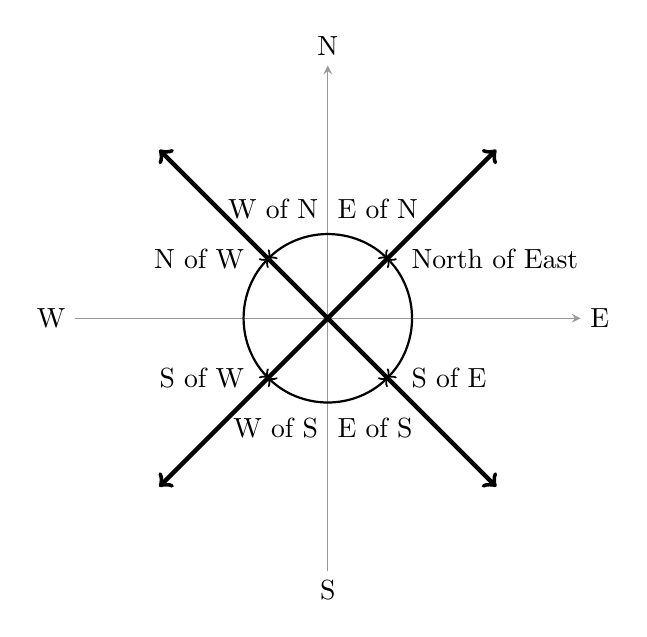
\begin{tikzpicture}
\pgfplotsset{compat=1.11}
    \begin{axis}[width=8cm, height=8cm,
        axis lines = middle,
        axis line style = {black!40},
        xlabel = E, x label style={anchor=west},
        ylabel = N, y label style={anchor=south},
        ymin=-3, ymax=3,
        xmin=-3, xmax=3,
        ticks=none,
        clip=false,
        ]
        \node[left] at (-3,0) {W};
        \node[below] at (0,-3) {S};
        \draw[ultra thick,<->] (-2,-2) -- (2,2);
        \draw[ultra thick,<->] (-2,2) -- (2,-2);
        \draw[thick,->] (1,0) arc (0:45:1) node[right=5pt] {North of East};
        \draw[thick,->] (0,1) arc (90:45:1);
        \draw[thick,->] (0,1) arc (90:135:1);
        \draw[thick,->] (-1,0) arc (180:135:1) node[left=5pt] {N of W};
        \draw[thick,->] (-1,0) arc (180:225:1) node[left=5pt] {S of W};
        \draw[thick,->] (0,-1) arc (270:225:1);
        \draw[thick,->] (0,-1) arc (270:315:1);
        \draw[thick,->] (1,0) arc (0:-45:1) node[right=5pt] {S of E};
        \node[right] at (0,1.3) {E of N};
        \node[left] at (0,1.3) {W of N};
        \node[left] at (0,-1.3) {W of S};
        \node[right] at (0,-1.3) {E of S};
    \end{axis}
\end{tikzpicture}
\end{minipage}%
\hspace{2em}
\begin{minipage}{0.5\textwidth}
\centering
    \begin{tabular}{c|c}
        \textbf{DO NOT USE} & \textbf{USE} \\
        \hline
        E of N & North of East\\
        W of N & N of W\\
        W of S & S of W\\
        E of S & S of E\\
    \end{tabular}
\end{minipage}

Two angles in the same quadrant are complimentary: they add up to \SI{90}{\degree}. For example, an \textbf{east of north} (E of N) angle is complementary to a \textbf{north of east} (N of E) angle. To convert degrees E of N to degrees N of E, calculate 90 minus the E of N angle. The same applies to other directions (e.g., W of S $\rightarrow$ S of W).

\subsection{Calculating Components Analytically}

Cosine (cos) and sine (sin) are trig functions on a calculator.

Cosine (cos) says, ``You give me the magnitude and direction (angle) of a vector; I give you the $x$-component.''.

Sine (cos) says, ``You give me the magnitude and direction (angle) of a vector; I give you the $y$-component.''

\begin{example}
    Vector $\vec{A}$ has a magnitude of 25 and is directed \SI{30}{\degree} north of east. (a) What is the $x$-component ($A_x$) of the vector? (b) What is the vector's $y$-component ($A_y$)?
\end{example}

\Solution Always sketch a picture to visualize the problem.

\begin{figure}[h!]
    \centering
\def\A{5}
\def\angle{30}
\begin{tikzpicture}
\pgfplotsset{compat=1.11}
\begin{axis}[width=8cm,height=8cm,
    axis lines=middle,
    axis line style={black!20},
    xmin=-5,xmax=5,ymin=-5,ymax=5,
    axis equal,
    ticks = none,
    xlabel = E, x label style={anchor=west},
    ylabel = N, y label style={anchor=south},
        ticks=none,
        clip=false,
        ]
        \node[left] at (axis cs: -5,0) {W};
        \node[below] at (axis cs: 0,-5) {S};
        \draw[thick] (axis cs: 1,0) arc (0:\angle:1);
        \node at (axis cs: 2,0.5) {\SI{\angle}{\degree}};
        \draw[ultra thick,black,->] (axis cs: 0,0) -- ++(axis direction cs: {\A*cos(\angle)},{\A*sin(\angle)}) node[right,align=left] {$\vec{A}=25$};
    \end{axis}
\end{tikzpicture}
\end{figure}

\textbf{Key idea}: The $x$-component ($A_x$) is equal to the magnitude of vector $\vec{A}$ multiplied by cosine (cos) of the angle from the $+x$-axis to the vector:

\begin{equation*}
    \vec{A}_x = 25 \cos{(\SI{30}{\degree})} = +21.65
\end{equation*}

(b) Likewise, the $y$-component ($A_y$) is equal to the magnitude of vector $\vec{A}$ multiplied by sine (sin) of the angle from the $+x$-axis to the vector:

\begin{equation*}
    \vec{A}_y = 25 \sin{(\SI{30}{\degree})} = +12.5
\end{equation*}

\textbf{Note}: Your calculator must be in ``degrees'' mode for these calculations to work.

\begin{example}
    Vector $\vec{A}$ has a magnitude of 49 at \SI{73}{\degree} north of west. Find the $x$- and $y$-components of $\vec{A}$.
\end{example}

\Solution The picture is

\begin{figure}[h!]
    \centering
\def\A{6}
\def\angle{73}
\begin{tikzpicture}
\pgfplotsset{compat=1.11}
\begin{axis}[width=8cm,height=8cm,
    axis lines=middle,
    axis line style={black!20},
    xmin=-6,xmax=6,ymin=-6,ymax=6,
    axis equal,
    ticks = none,
    xlabel = E, x label style={anchor=west},
    ylabel = N, y label style={anchor=south},
        ticks=none,
        clip=false,
        ]
        \node[left] at (-6,0) {W};
        \node[below] at (0,-6) {S};
        \draw[thick] (-1,0) arc (180:180-\angle:1);
        \node at (-1.1,1) {\SI{\angle}{\degree}};
        \draw[ultra thick,black,->] (0,0) -- ({-\A*cos(\angle)},{\A*sin(\angle)}) node[above] {$\vec{A} = 49$};
        \draw[dashed,thick,->] (0,0) -- ({-\A*cos(\angle)},0) node[below] {$\vec{A}_x$}; 
        \draw[dashed,thick,->] ({-\A*cos(\angle)},0) -- ({-\A*cos(\angle)},{\A*sin(\angle)}) node[below left] {$\vec{A}_y$}; 
    \end{axis}
\end{tikzpicture}%
\hspace{2em}
\begin{tikzpicture}
\pgfplotsset{compat=1.11}
\begin{axis}[width=8cm,height=8cm,
    axis lines=middle,
    axis line style={black!20},
    xmin=-6,xmax=6,ymin=-6,ymax=6,
    % axis equal,
    ticks = none,
    xlabel = E, x label style={anchor=west},
    ylabel = N, y label style={anchor=south},
        ticks=none,
        clip=false,
        ]
        \node[left] at (-6,0) {W};
        \node[below] at (0,-6) {S};
        \draw[thick] (-1,0) arc (180:180-\angle:1);
        \draw[thick,red] (1,0) arc (0:180-\angle:1);
        \node[red] at (0.7,1.4) {$\beta$};
        \node at (-1.5,0.8) {\SI{\angle}{\degree}};
        \draw[ultra thick,black,->] (0,0) -- ({-\A*cos(\angle)},{\A*sin(\angle)}) node[left] {$\vec{A} = 49$};
    \end{axis}
\end{tikzpicture}
\end{figure}

The given angle, \SI{73}{\degree}, is measured from the $-x$ axis, so it's not in standard position; its application calculates only the \textit{magnitude} (not direction) of $x$- and $y$-components: 


\begin{align*}
    A_x &= 49 \cos{(73)} = 14.3\\[1ex]
    A_y &= 49 \sin{(73)} = 46.9
\end{align*}


Directions are inferred by noting that the $x$-component vector points left, towards the $-x$ axis, making $A_x$ negative, and that the $y$-component vector, pointing towards $+y$, is positive:

\begin{equation*}
    \vec{A}_x = -14.3\ , \hspace{1em}
    \vec{A}_y = +46.9
\end{equation*}

An alternative solution: Only angles in standard position yield both magnitude and direction. Here, the \href{https://mathworld.wolfram.com/SupplementaryAngles.html}{supplementary angle} of \SI{73}{\degree} ($\beta$ in the figure) \textit{is} in standard position and is found by

\begin{equation*}
    \beta = 180 - 73 = \SI{107}{\degree}
\end{equation*}

The vector components are

\begin{align*}
    \vec{A}_x &= 49 \cos{(107)} = -14.3\\[1ex]
    \vec{A}_y &= 49 \sin{(107)} = +46.9
\end{align*}

\hrule

\begin{example}
    Hedwig the Owl starts at his nest and undergoes a displacement of 12 kilometers at \SI{32}{\degree} east of north. (a) What is the $x$-component (East) of his displacement? (b) What is the $y$-component (North)?
\end{example}

\Solution

\begin{figure}[h!]
    \centering
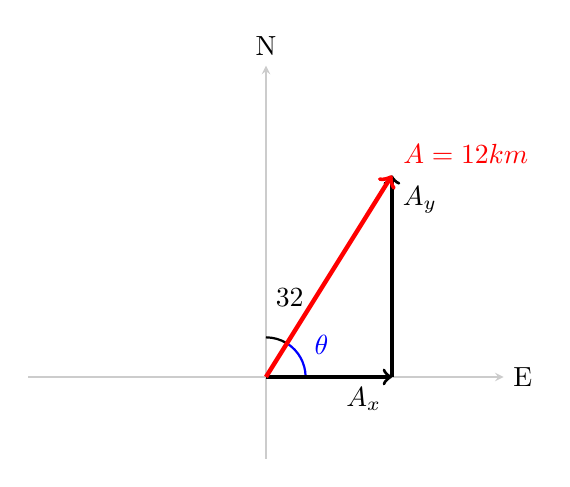
\begin{tikzpicture}
\def\A{3}
\def\angle{58}
\pgfplotsset{compat=1.11}
\begin{axis}[width=3in,
    axis lines=middle,
    xmin=-3,xmax=3,ymin=-0.1,ymax=3,
    axis equal,
    ticks = none,
    xlabel = E, x label style={anchor=west},
    ylabel = N, y label style={anchor=south},
    axis line style={black!20},
    clip=false,
    ]
    \draw[thick,blue] (0.5,0) arc (0:\angle:0.5);
    \node[blue] at (0.7,0.4) {$\theta$};
    \draw[->,very thick] (0,0) -- ({\A*cos(\angle)},0) node[below left] {$A_x$};
    \draw[->,very thick] ({\A*cos(\angle)},0) -- ({\A*cos(\angle)},{\A*sin(\angle)}) node[below right] {$A_y$};
    \draw[thick] (0,0.5) arc (90:58:0.5);
    \node at (0.3,1) {\SI{32}{\degree}};
    \draw[->,ultra thick,red] (0,0) -- ({\A*cos(\angle)},{\A*sin(\angle)}) node[above right] {$A=\SI{12}{km}$};
\end{axis}
\end{tikzpicture}
\end{figure}

Do not use the E of N angle of \SI{32}{\degree}. Convert it to N of E as follows:

\begin{equation*}
    \theta = \SI{90}{\degree} - \SI{32}{\degree} = \SI{58}{\degree}
\end{equation*}

The angle $\theta = \SI{58}{\degree}$, which is in standard position, may now be used in our $\cos$ and $\sin$ functions.

(a) The $x$-component equals the magnitude of the vector times the cosine of the angle:

\begin{equation*}
    \vec{A}_x = 12 \cos{(58)} = +\SI{6.36}{km}
\end{equation*}

(b) The $y$-component is

\begin{equation*}
    \vec{A}_y = 12 \sin{(58)} = +\SI{10.18}{km}
\end{equation*}

\hrule

\begin{example}
    The Eiffel Tower is \SI{789}{ft} and \SI{114}{\degree} from Jarred the tourist. (a) How far north is the Eiffel tower? (b) How far west?
\end{example}

\Solution

\begin{figure}[h!]
    \centering
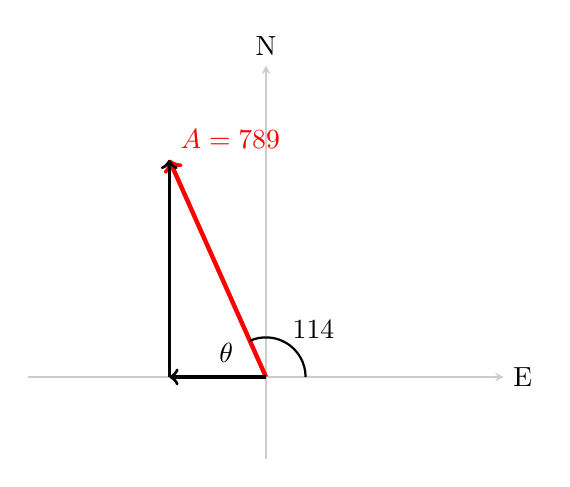
\begin{tikzpicture}
\def\A{3}
\def\angle{114}
\pgfplotsset{compat=1.11}
\begin{axis}[width=3in,
    axis lines=middle,
    xmin=-3,xmax=3,ymin=-0.1,ymax=3,
    axis equal,
    ticks = none,
    xlabel = E, x label style={anchor=west},
    ylabel = N, y label style={anchor=south},
    axis line style={black!20},
    ]
    \draw[->,ultra thick,red] (0,0) -- ({\A*cos(\angle)},{\A*sin(\angle)}) node[above right] {$A=789$};
    \draw[thick] (0.5,0) arc (0:\angle:0.5);
    \node at (0.6,0.6) {\SI{114}{\degree}};
    \draw[->,very thick] (0,0) -- ({\A*cos(\angle)},0);
    \draw[->,very thick] ({\A*cos(\angle)},0) -- ({\A*cos(\angle)},{\A*sin(\angle)});
    \node at (-0.5,0.3) {$\theta$};
\end{axis}
\end{tikzpicture}
\end{figure}

The angle $\theta$ is

\begin{equation*}
    \theta = \SI{180}{\degree} - \SI{114}{\degree} = \SI{66}{\degree}
\end{equation*}

(a) The magnitude of the $x$-component is 

\begin{equation*}
    A_x = 789 \cos{(66)} = \SI{320.9}{ft}
\end{equation*}

Therefore, the Eiffel Tower is \SI{320.9}{ft} west.

(b) The magnitude of the $y$-component is

\begin{equation*}
    A_y = 789 \sin{(66)} = \SI{720.8}{ft}
\end{equation*}

Therefore, it's \SI{720.8}{ft} north.

An alternative solution: The standard position angle $\SI{114}{\degree}$ directly yields 

\begin{align*}
    \vec{A}_x &= 789 \cos{(114)} = -\SI{320.9}{ft}\\[1ex]
    \vec{A}_y &= 789 \sin{(114)} = +\SI{720.8}{ft}
\end{align*}

\begin{example}
    Pac-Man takes 3 steps to the right and 4 steps up. (a) What is the magnitude of his resultant displacement vector? (b) What is the direction of the resultant vector?
\end{example}

\Solution The picture is

\begin{figure}[h!]
    \centering
\begin{tikzpicture}
\def\A{7}
\def\angle{53.13}
\pgfplotsset{compat=1.11}
\begin{axis}[width=8cm,
    axis lines=middle,
    xmin=-1,xmax=7,ymin=-1,ymax=7,
    axis equal,
    ticks = none,
    xlabel = E, x label style={anchor=west},
    ylabel = N, y label style={anchor=south},
    axis line style={black!20},
    clip=false,
    ] 
    \draw[thick,->] (0,0) -- ({\A*cos(\angle)},0) node[below] {$\vec{A}_x = 3$};
    \draw[thick,->] ({\A*cos(\angle)},0) -- ++(axis direction cs: 0,{\A*sin(\angle)}) node[right] {$\vec{A}_y = 4$};
    \draw[ultra thick,->,red] (0,0) -- ({\A*cos(\angle)},{\A*sin(\angle)}) node[above left] {$\vec{A}$};
    \draw[thick] (1,0) arc (0:\angle:1);
    \node at (1.3,0.6) {$\theta$};
    \end{axis}
\end{tikzpicture}
\end{figure}

(a) The \href{https://mathworld.wolfram.com/PythagoreanTheorem.html}{Pythagorean theorem} ($a^2 + b^2 = c^2$) relates the three sides of a right triangle. Since vector $\vec{A}$ and its components form a right triangle, it follows that the magnitude of $\vec{A}$ is given by

\begin{equation*}
    3^2 + 4^2 = A^2
\end{equation*}

To solve for $A$, the magnitude of the vector, take the square root of both sides:

\begin{equation*}
    A = \sqrt{3^2 + 4^2} = 5
\end{equation*}

(b) The direction, given by $\theta$, is found by taking the inverse tangent (another trig function) of the $y$-component divided by the $x$-component:

\begin{equation*}
    \theta = \tan^{-1}\left(\frac{4}{3}\right) = \SI{53.1}{\degree}
\end{equation*}

\hrule

\clearpage

\begin{mdframed}[backgroundcolor=black!10]
\textit{Vector summary}. In general, consider vector $\vec{A}$, of magnitude $A$, whose direction is given by an angle $\theta$ that is in standard position. The $x$- and $y$-components of $\vec{A}$, the magnitude of $\vec{A}$, and the directional angle $\theta$ are generally given by the following relations: 

\begin{equation*}
    \vec{A}_x = A \cos{\theta}\ , \hspace{1em}
    \vec{A}_y = A \sin{\theta}\ , \hspace{1em}
    A = \sqrt{A_x^2 + A_y^2}\ , \hspace{1em}
    \theta = \tan^{-1}\left(\frac{A_y}{A_x}\right)
\end{equation*}
\end{mdframed}

\begin{figure}[h!]
    \centering
    \pgfplotsset{compat=1.11}
    \def\A{6}
    \def\angle{55}
\begin{tikzpicture}
    \begin{axis}[width=8cm,height=8cm,
        axis lines=middle,
        axis line style={black!20},
        xmin=-6,xmax=6,
        ymin=-6,ymax=6,
        clip=false,
        ticks=none,
        xlabel=$+x$,
        x label style={anchor=west},
        ylabel=$+y$, y label style={anchor=south},
    ]
    \draw[thick,->] (0,0) -- ({\A*cos(\angle)},0) node[below] {$\vec{A}_x$};
    \draw[thick,->] ({\A*cos(\angle)},0) -- ({\A*cos(\angle)},{\A*sin(\angle)}) node[below right] {$\vec{A}_y$};
    \draw[ultra thick,red,->] (0,0) -- ({\A*cos(\angle)},{\A*sin(\angle)}) node[above,red] {$\vec{A}$};
    \draw[thick] (1,0) arc (0:\angle:1); 
    \node at (1.3,0.7) {$\theta$};
    \end{axis}
\end{tikzpicture}
\end{figure}

\begin{example}
    Alice undergoes two displacements: 49 meters east and 67 meters north. Her third displacement gets her back to the initial position. (a) What is the magnitude of the resultant (3rd) displacement vector? (b) What is the direction as measured from \SI{0}{\degree} (i.e., from $+x$ or East)?
\end{example}

\Solution It's helpful to draw two pictures. The first shows the $x$- and $y$ components and the resultant vector $R$ that leads back to the origin.

\begin{figure}[h!]
    \centering
\begin{tikzpicture}
\def\A{3}
\def\angle{53.82}
\pgfplotsset{compat=1.11}
\begin{axis}[width=8cm,
    axis lines=middle,
    xmin=-3,xmax=3,ymin=-3,ymax=3,
    axis equal,
    ticks = none,
    xlabel = E, x label style={anchor=west},
    ylabel = N, y label style={anchor=south},
    axis line style={black!20},
    clip=false
    ]
    \draw[->,ultra thick,red]  ({\A*cos(\angle)},{\A*sin(\angle)}) -- (0,0);
    \node[red] at (0.3,0.9) {$R$};
    \draw[thick] (0.7,0) arc (0:\angle:0.7);
    \node at (0.9,0.35) {$\alpha$};
    \draw[->,very thick] (0,0) -- ({\A*cos(\angle)},0) node[below] {\SI{49}{m}};
    \draw[->,very thick] ({\A*cos(\angle)},0) -- ({\A*cos(\angle)},{\A*sin(\angle)}) node[right] {\SI{67}{m}};
\end{axis}
\end{tikzpicture}%
\hfill
\begin{tikzpicture}
\def\A{3}
\def\angle{53.82}
\pgfplotsset{compat=1.11}
\begin{axis}[width=8cm,
    axis lines=middle,
    xmin=-3,xmax=3,ymin=-3,ymax=3,
    axis equal,
    ticks = none,
    xlabel = E, x label style={anchor=west},
    ylabel = N, y label style={anchor=south},
    axis line style={black!20},
    clip=false
    ]
    \begin{scope}[xshift=-1.57cm,yshift=-2.13cm]
    \draw[->,ultra thick,red] ({\A*cos(\angle)},{\A*sin(\angle)}) -- (0,0);
    \node[red] at (0.3,-0.3) {$R$};
    \draw[dashed] (0,0) -- (1.2,0);
    \draw[thick] (0.6,0) arc (0:\angle:0.6);
    \node at (0.8,0.35) {$\alpha$};
    \end{scope}
    \draw[thick] (-0.5,0) arc (180:180+\angle:0.5);
    \node at (-0.65,-0.3) {$\alpha$};
    \draw[thick,blue,->] (1,0) arc (0:180+\angle:1);
    \node[blue] at (-0.5,1.2) {$\theta$};
\end{axis}
\end{tikzpicture}
\end{figure}

The magnitude of the resultant is

\begin{equation*}
    R = \sqrt{49^2 + 67^2} = \SI{83}{m}
\end{equation*}

(b) Angle $\alpha$, while \textit{not} the desired angle, is necessary to find direction and is calculated as

\begin{equation*}
    \alpha = \tan^{-1}\left(\frac{67}{49}\right) = \SI{53.8}{\degree}
\end{equation*}

In the second picture, vector $\vec{R}$ is re-centered at standard position. Since $\vec{R}$ is in quadrant III, it's direction ($\theta$) is \SI{180}{\degree} (from quadrants I and II) plus $\alpha$:

\begin{equation*}
    \theta = 180 + \alpha = 180 + 53.8 = \SI{233.8}{\degree}\ .
\end{equation*}


\subsection{Horizontally Launched Projectiles}

\begin{figure}[h!]
    \centering
    \begin{tabular}{cl|cl}
    \hline
    \textbf{Symbol} & \textbf{Quantity} & \textbf{Unit} & \textbf{Unit Symbol}  \\
    \hline\hline
        $d_x$ & horizontal displacement (or position) & meter & m\\
        $d_y$ & vertical displacement (or position) & meter & m\\
        $t$ & time & second & s\\
        $v$ & velocity & meter per second & m/s\\
        $v_0$ & initial velocity & meter per second & m/s\\
        $v_{0y}$ & vertical component of initial velocity & meter per second & m/s\\
        $v_{0x}$ & horizontal component of initial velocity & meter per second & m/s\\
        $v_y$ & vertical velocity & meter per second & m/s\\
        $v_x$ & horizontal velocity & meter per second & m/s\\
        $a_y$ & vertical component of acceleration & meter per second squared & $\SI{}{m/s^2}$\\
        $g$ & acceleration due to gravity & meter per second squared & \SI{}{m/s^2}\\
        % $\theta$ & projectile \textbf{instantaneous} angle & degrees & \SI{}{\degree}\\
        % $\theta_0$ & projectile \textbf{launch} angle & degrees & \SI{}{\degree}\\
        % $y_{\mathrm{max}}$ & maximum projectile height & meter & m\\
        % $t_{\mathrm{max}}$ & time from launch to $y_{\mathrm{max}}$ & second & s\\
        % $R$ & projectile range & meter & m\\
    \hline
    \end{tabular}
    % \caption*{Symbols and units of physical quantities in projectile motion. As you read the information below, refer back to this table frequently to review what a symbol means.}
    \label{fig:my_label}
\end{figure}

Projectile motion is the motion of an object thrown into the air. The object,known as the ``projectile,'' experiences only downward acceleration due to gravity. The trajectory is the curved path of a projectile through the air. In projectile motion, horizontal and vertical motions (e.g., displacement, velocity, acceleration) are independent: their $x$- and $y$-components don't influence each other. For example, a projectile's $\vec{v}_x$ vector can be analyzed separately from its $\vec{v}_y$.

A \textit{horizontally launched projectile} is an object that is thrown with an initial velocity that is entirely horizontal. In such a case, the $y$-component of the initial velocity is zero, and the $x$-component of initial velocity is the velocity at which the object is launched. 

\begin{mdframed}[backgroundcolor=black!10]
The horizontal motion of a horizontally launched projectile is governed by these equations:
\vspace{-1em}

\begin{align*}
    \vec{a}_x &= 0\\[0.5ex]
    \vec{v}_x &= \mathrm{constant} = \vec{v}_{0x}\\[0.5ex]
    \vec{d}_x &= \vec{v}_{0x} \cdot t\\[0.5ex]
\end{align*}
\vspace{-3em}

\begin{center}
        \begin{tabular}{cl|cl}
    \hline
    \textbf{Symbol} & \textbf{Quantity} & \textbf{Unit} & \textbf{Unit Symbol}  \\
    \hline\hline
        $a_x$ & horizontal component of acceleration & meter per second squared & $\SI{}{m/s^2}$\\
        $v_x$ & horizontal velocity & meter per second & m/s\\
        $v_{0x}$ & horizontal component of initial velocity & meter per second & m/s\\
        $d_x$ & horizontal displacement (or position) & meter & m\\
        $t$ & time & second & s\\
    \hline
    \end{tabular}
\end{center}
% \textbf{Note}: The velocity at which the projectile is launched is the same as $\vec{v}_{0x}$.
\end{mdframed}

\begin{mdframed}[backgroundcolor=black!10]
After launch, the projectile accelerates downward due to gravity. The magnitude of this acceleration is

\begin{equation*}
    g = \SI{9.8}{m/s^2}\ .
\end{equation*}
\end{mdframed}

\begin{mdframed}[backgroundcolor=black!10]
The \textit{vertical} motion of a horizontally launched projectile is governed by these equations:
\vspace{-1em}

\begin{align*}
    \vec{a}_y &= -g = -\SI{9.8}{m/s^2}\\
    \vec{v}_y &= - gt\\
    \vec{d}_y &= -\frac{1}{2} g t^2\\
\end{align*}
\vspace{-3em}

\begin{center}
    \begin{tabular}{cl|cl}
    \hline
    \textbf{Symbol} & \textbf{Quantity} & \textbf{Unit} & \textbf{Unit Symbol}  \\
    \hline\hline
        $a_y$ & vertical component of acceleration & meter per second squared & $\SI{}{m/s^2}$\\
        $v_y$ & vertical velocity & meter per second & m/s\\
        $v_{0y}$ & vertical component of initial velocity & meter per second & m/s\\
        $d_y$ & vertical displacement (or position) & meter & m\\
        $t$ & time & second & s\\
    \hline
    \end{tabular}
\end{center}
\end{mdframed}

% Range is

% \begin{equation*}
%     R = \frac{v^2_0 \sin{2\theta_0}}{g}\ .
% \end{equation*}

% The equation of the path is

% \begin{equation*}
%     y =  -\frac{g x^2}{2\left(v_0 \cos{\theta_0}\right)^2} + \left(\tan{\theta_0}\right) x + y_0
% \end{equation*}

\begin{example} \label{r4IUyp}
    A metallic ball is shot horizontally at \SI{12}{m/s} from the top of a tall cliff. (a) Calculate horizontal components of velocity at 1-second time intervals for the first 5 seconds of motion. (b) Do the same for vertical components.
\end{example}

\begin{figure}[h!]
    \centering
    \begin{tikzpicture} 
    \tikzmath{
        \gravity = 9.8;
        \vi = 28.6;
        \yi = 60;
        \thetai = 0.0;
        \ys = 1.3;
    }
    \pgfplotsset{compat=1.11}
        \begin{axis}[width=6cm,height=6cm,ticks=none,
        axis line style = {black!50},
        axis lines = middle,
        clip=false,
        ylabel style= {anchor=south},
        xlabel style= {anchor=west},
        ylabel = $y$,
        xlabel = $x$,
        xmin=0, xmax=120,
        ymin=0, ymax=80,
        ]
        \addplot [dashed,
            domain=0:100,
            samples=100, 
            color=black!50,
        ]
        {\yi + tan(\thetai)*x - \gravity*x^2/(2*(\vi*cos(\thetai))^2)}; %equation of path
        \fill (0,\yi) circle (2pt) node[left] {$y_0$};
        \draw[thick,->,red] (0,\yi) -- (12,\yi) node[above] {$v_x$};
        \fill (20,57.60) circle (2pt); %Calculated using equator of path
        \draw[thick,->,red] (20,57.60) -- ++(axis direction cs: 12,0) node[above] {$v_x$};
        \draw[thick,->,red] (20,57.60) -- ++(axis direction cs: 0,-5*\ys^0) node[left] {$v_y$};
        \fill (40,50.42) circle (2pt);
        \draw[thick,->,red] (40,50.42) -- ++(axis direction cs: 12,0) node[above] {$v_x$};
        \draw[thick,->,red] (40,50.42) -- ++(axis direction cs: 0,-5*\ys^1) node[left] {$v_y$};
        \fill (60,38.43) circle (2pt);
        \draw[thick,->,red] (60,38.43) -- ++(axis direction cs: 12,0) node[above] {$v_x$};
        \draw[thick,->,red] (60,38.43) -- ++(axis direction cs: 0,-5*\ys^2) node[left] {$v_y$};
        \fill (80,21.66) circle (2pt);
        \draw[thick,->,red] (80,21.66) -- ++(axis direction cs: 12,0) node[above] {$v_x$};
        \draw[thick,->,red] (80,21.66) -- ++(axis direction cs: 0,-5*\ys^3) node[left] {$v_y$};
        \fill ({\vi*sqrt(2*\yi/\gravity)},0) circle (2pt) node[below left] {$x_f$};
        \draw[thick,->,red] ({\vi*sqrt(2*\yi/\gravity)},0) -- ++(axis direction cs: 12,0) node[above] {$v_x$};
        \draw[thick,->,red] ({\vi*sqrt(2*\yi/\gravity)},0) -- ++(axis direction cs: 0,-5*\ys^4) node[left] {$v_y$};
        \end{axis}
    \end{tikzpicture}
\end{figure}

\Solution (a) We are given initial velocity: $v_0 = \SI{12}{m/s}$. Since $v_0$ is entirely horizontal, the $x$-component of $v_0$ is also \SI{12}{m/s}:

\begin{equation*}
    \vec{v}_{0x} = +\SI{12}{m/s}
\end{equation*}

For horizontal motion, acceleration is zero:

\begin{equation*}
    a_x = 0\ .
\end{equation*}

Zero horizontal acceleration implies no change in horizontal velocity:
\vspace{-1em}

\begin{align*}
    v_x \text{ at \SI{1.0}{s}} &= \SI{12}{m/s}\\[0.5ex]
    v_x \text{ at \SI{2.0}{s}} &= \SI{12}{m/s}\\[0.5ex]
    v_x \text{ at \SI{3.0}{s}} &= \SI{12}{m/s}\\[0.5ex]
    v_x \text{ at \SI{4.0}{s}} &= \SI{12}{m/s}\\[0.5ex]
    v_x \text{ at \SI{5.0}{s}} &= \SI{12}{m/s}\\[0.5ex]
\end{align*}

(b) Recall that the magnitude of acceleration due to gravity is $g = \SI{9.8}{m/s^2}$. The vertical component of velocity for a horizontally launched projectile is 

\begin{equation*} 
    v_y = -g t = -9.8 t
\end{equation*}

Therefore, vertical velocities are

\begin{align*}
    v_y \text{ at \SI{1.0}{s}} &= (-9.8)(1) = \SI{-9.8}{m/s}\\[0.5ex]
    v_y \text{ at \SI{2.0}{s}} &= (-9.8)(2) = \SI{-19.6}{m/s}\\[0.5ex]
    v_y \text{ at \SI{3.0}{s}} &= (-9.8)(3) = \SI{-29.4}{m/s}\\[0.5ex]
    v_y \text{ at \SI{4.0}{s}} &= (-9.8)(4) = \SI{-39.2}{m/s}\\[0.5ex]
    v_y \text{ at \SI{5.0}{s}} &= (-9.8)(5) = \SI{-49.0}{m/s}\\[0.5ex]
\end{align*}

\begin{example}
    For the projectile in Example~\ref{r4IUyp}, (a) calculate horizontal components of displacement at 1-second time intervals for 5 seconds. (b) Do the same for vertical components of displacement.
\end{example}

\begin{figure}[h!]
    \centering
    \begin{tikzpicture} 
    \tikzmath{
        \gravity = 9.8;
        \vi = 28.6;
        \yi = 60;
        \thetai = 0.0;
        \ys = 1.3;
        \x1 = 20; \y1 = 57.60;
        \x2 = 40; \y2 = 50.42;
        \x3 = 60; \y3 = 38.43;
        \x4 = 80; \y4 = 21.66;
        \x5 = \vi*sqrt(2*\yi/\gravity); \y5 = 0;
    }
    \pgfplotsset{compat=1.11}
        \begin{axis}[width=8cm,height=8cm,ticks=none,
        axis line style = {black!50},
        axis lines = middle,
        clip=false,
        ylabel style= {anchor=south},
        xlabel style= {anchor=west},
        ylabel = $y$,
        xlabel = $x$,
        xmin=0, xmax=120,
        ymin=0, ymax=80,
        ]
        \addplot [dashed,
            domain=0:100,
            samples=100, 
            color=black!50,
        ]
        {\yi + tan(\thetai)*x - \gravity*x^2/(2*(\vi*cos(\thetai))^2)}; %equation of path
        \fill (0,\yi) circle (3pt) node[left] {$y_0$};
        \fill (\x1,\y1) circle (3pt); %Calculated using equator of path
        \draw[->,thick,red!80,dashed] (0,\y1) -- ++(axis direction cs: \x1,0) node[below left] {$d_x$};
        \draw[->,red] (\x1,\yi) -- ++(axis direction cs: 0,\y1-\yi) node[above right] {$d_y$};
        \fill (\x2,\y2) circle (3pt);
        \draw[->,thick,red!80,dashed] (0,\y2) -- ++(axis direction cs: \x2,0) node[below left] {$d_x$};
        \draw[->,thick,red!80,dashed] (\x2,\yi) -- ++(axis direction cs: 0,\y2-\yi) node[above right] {$d_y$};
        \fill (\x3,\y3) circle (3pt);
        \draw[->,thick,red!80,dashed] (0,\y3) -- ++(axis direction cs: \x3,0) node[below left] {$d_x$};
        \draw[->,thick,red!80,dashed] (\x3,\yi) -- ++(axis direction cs: 0,\y3-\yi) node[above right] {$d_y$};
        \fill (\x4,\y4) circle (3pt);
        \draw[->,thick,red!80,dashed] (0,\y4) -- ++(axis direction cs: \x4,0) node[below left] {$d_x$};
        \draw[->,thick,red!80,dashed] (\x4,\yi) -- ++(axis direction cs: 0,\y4-\yi) node[above right] {$d_y$};
        \fill (\x5,\y5) circle (3pt);
        \draw[->,thick,red!80,dashed] (0,\y5) -- ++(axis direction cs: \x5,0) node[below left] {$d_x$};
        \draw[->,thick,red!80,dashed] (\x5,\yi) -- ++(axis direction cs: 0,\y5-\yi) node[above right] {$d_y$};
        \end{axis}
    \end{tikzpicture}
\end{figure}

\Solution (a) Initial velocity is

\begin{equation*}
    v_0 = v_{0x} = \SI{12}{m/s}
\end{equation*}

Horizontal displacement is given by

\begin{equation*}
    d_x = v_{0x} \cdot t
\end{equation*}

The components are

\begin{align*}
    d_x \text{ at \SI{1.0}{s}} &= (\SI{12}{m/s})(\SI{1.0}{s}) = \SI{12}{m}\\[0.5ex]
    d_x \text{ at \SI{2.0}{s}} &= (\SI{12}{m/s})(\SI{2.0}{s}) = \SI{24}{m}\\[0.5ex]
    d_x \text{ at \SI{3.0}{s}} &= (\SI{12}{m/s})(\SI{3.0}{s}) = \SI{36}{m}\\[0.5ex]
    d_x \text{ at \SI{4.0}{s}} &= (\SI{12}{m/s})(\SI{4.0}{s}) = \SI{48}{m}\\[0.5ex]
    d_x \text{ at \SI{5.0}{s}} &= (\SI{12}{m/s})(\SI{5.0}{s}) = \SI{60}{m}\\[0.5ex]
\end{align*}

(b) Recalling that $g=\SI{9.8}{m/s^2}$,  the vertical displacement is given by

\begin{equation*}
    d_y = -\frac{1}{2} g t^2 = -\frac{1}{2}(9.8) t^2 = -4.9 t^2
\end{equation*}

Vertical displacements are
\vspace{-2em}

\begin{align*}
    d_y \text{ at \SI{1.0}{s}} &= -(4.9)(1^2) = -\SI{4.9}{m}\\[0.5ex]
    d_y \text{ at \SI{2.0}{s}} &= -(4.9)(2^2) = -\SI{19.6}{m}\\[0.5ex]
    d_y \text{ at \SI{3.0}{s}} &= -(4.9)(3^2) = -\SI{44.1}{m}\\[0.5ex]
    d_y \text{ at \SI{4.0}{s}} &= -(4.9)(4^2) = -\SI{78.4}{m}\\[0.5ex]
    d_y \text{ at \SI{5.0}{s}} &= -(4.9)(5^2) = -\SI{122.5}{m}\\[0.5ex]
\end{align*}
\vspace{-1em}

\begin{example} \label{i3PZ3N}
    Pel\'{e} kicks a soccer ball horizontally at a speed of \SI{30}{m/s} from the top of a building that is 500 meters tall. How long does the ball take to impact the ground?
\end{example}

\begin{figure}[h!]
    \centering
    \begin{tikzpicture} 
    \tikzmath{
        \gravity = 9.8;
        \vi = 28.6;
        \yi = 60;
        \thetai = 0.0;
        \ys = 1.3;
        \x1 = 20; \y1 = 57.60;
        \x2 = 40; \y2 = 50.42;
        \x3 = 60; \y3 = 38.43;
        \x4 = 80; \y4 = 21.66;
        \x5 = \vi*sqrt(2*\yi/\gravity); \y5 = 0;
    }
    \pgfplotsset{compat=1.11}
        \begin{axis}[width=6cm,height=6cm,ticks=none,
        axis line style = {black!50},
        axis lines = middle,
        clip=false,
        ylabel style= {anchor=south},
        xlabel style= {anchor=west},
        ylabel = $y$,
        xlabel = $x$,
        xmin=0, xmax=120,
        ymin=0, ymax=80,
        ]
        \addplot [dashed,
            domain=0:100,
            samples=100, 
            color=black!50,
        ]
        {\yi + tan(\thetai)*x - \gravity*x^2/(2*(\vi*cos(\thetai))^2)}; %equation of path
        \fill (0,\yi) circle (2pt);% node[left] {$y_0$};
        \fill (\x1,\y1) circle (2pt); %Calculated using equator of path
        \fill (\x2,\y2) circle (2pt);
        \fill (\x3,\y3) circle (2pt);
        \fill (\x4,\y4) circle (2pt);
        \fill (\x5,\y5) circle (2pt);
        \end{axis}
    \end{tikzpicture}
\end{figure}

\Solution The impact time depends on the height from which the ball drops. This height is the magnitude of the ball's vertical displacement ($d_y$):

\begin{equation*}
    d_y = -\frac{1}{2} g t^2\ \hspace{2em} (\text{where } g = \SI{9.8}{m/s^2})\ .
\end{equation*}

The ball drops 500 meters, so it's vertical displacement is $d_y = \SI{-500}{m}$. Plugging in values into the equation above leads to

\begin{equation*}
    -500 = -\frac{1}{2} (9.8) t^2 = -4.9 t^2\ ,
\end{equation*}

or, eliminating the negative signs,

\begin{equation*}
    500 = 4.9 t^2\ .
\end{equation*}

To find impact time, we solve this equation for time $t$ as follows:

\begin{align*}
    % \hspace{-10em} \textbf{Multiply $\frac{1}{2}$ by 9.8} 
    % \hspace{5em} & 500 = \frac{1}{2} (9.8) t^2\\[1ex] 
    % \hspace{-10em} \textbf{Simplify} \hspace{5em} & 500 = 4.9 t^2\\[1ex] 
   \hspace{-10em} \textbf{Divide by $4.9$} \hspace{5em} & \frac{500}{\textcolor{red}{4.9}} = \frac{\cancel{4.9}\,t^2}{\textcolor{red}{\cancel{4.9}}}\\[1ex] 
    \hspace{-10em} \textbf{Simplify} \hspace{5em} & 102 = t^2\\[1ex] 
    \hspace{-10em} \textbf{Put $t$ on the left} \hspace{5em} & t^2 = 102\\[1ex] 
    \hspace{-10em} \textbf{Take square root} \hspace{5em} & \sqrt{t^2} = \sqrt{102} = 10.1\\[1ex] 
\end{align*}

Therefore, the time the ball will take to impact the floor is

\begin{equation*}
    t = \SI{10.1}{s}\ .
\end{equation*}

\begin{example}
   For the ball in Example~\ref{i3PZ3N}, what is the magnitude of the velocity the instant the ball impacts the ground? This is known as the ``entry speed.'' 
\end{example}

\begin{figure}[h!]
    \centering
    \begin{tikzpicture} 
    \tikzmath{
        \gravity = 9.8;
        \vi = 28.6;
        \yi = 60;
        \thetai = 0.0;
        \ys = 1.3;
    }
    \pgfplotsset{compat=1.11}
        \begin{axis}[width=8cm,height=8cm,ticks=none,
        axis line style = {black!20},
        axis lines = middle,
        clip=false,
        ylabel style= {anchor=south},
        xlabel style= {anchor=west},
        ylabel = $y$,
        xlabel = $x$,
        xmin=0, xmax=120,
        ymin=-80, ymax=80,
        ]
        \addplot [dashed,
            domain=0:100,
            samples=100, 
            color=black!50,
        ]
        {\yi + tan(\thetai)*x - \gravity*x^2/(2*(\vi*cos(\thetai))^2)}; %equation of path
        \fill (0,\yi) circle (2pt) node[left] {$t=0$};
        % \draw[thick,->,red] (0,\yi) -- (12,\yi) node[above] {$v_x$};
        % \fill (20,57.60) circle (2pt); %Calculated using equator of path
        % \draw[thick,->,red] (20,57.60) -- ++(axis direction cs: 12,0) node[above] {$v_x$};
        % \draw[thick,->,red] (20,57.60) -- ++(axis direction cs: 0,-5*\ys^0) node[left] {$v_y$};
        % \fill (40,50.42) circle (2pt);
        % \draw[thick,->,red] (40,50.42) -- ++(axis direction cs: 12,0) node[above] {$v_x$};
        % \draw[thick,->,red] (40,50.42) -- ++(axis direction cs: 0,-5*\ys^1) node[left] {$v_y$};
        % \fill (60,38.43) circle (2pt);
        % \draw[thick,->,red] (60,38.43) -- ++(axis direction cs: 12,0) node[above] {$v_x$};
        % \draw[thick,->,red] (60,38.43) -- ++(axis direction cs: 0,-5*\ys^2) node[left] {$v_y$};
        % \fill (80,21.66) circle (2pt);
        % \draw[thick,->,red] (80,21.66) -- ++(axis direction cs: 12,0) node[above] {$v_x$};
        % \draw[thick,->,red] (80,21.66) -- ++(axis direction cs: 0,-5*\ys^3) node[left] {$v_y$};
        \fill ({\vi*sqrt(2*\yi/\gravity)},0) circle (2pt) node[below left=5pt,align=left] {impact\\ $t=10.1$};
        \draw[thick,->,red] ({\vi*sqrt(2*\yi/\gravity)},0) -- ++(axis direction cs: 12,0) node[above] {$v_x$};
        \draw[thick,->,red] ({\vi*sqrt(2*\yi/\gravity)},0) -- ++(axis direction cs: 0,-40) node[left] {$v_y$};
        \end{axis}
    \end{tikzpicture}
\end{figure}

\Solution The horizontal velocity at impact is the same as its initial value:

\begin{equation*}
    v_x = v_{0x} = +\SI{30}{m/s}
\end{equation*}

As calculated in the previous example, impact occurs at time $t=\SI{10.1}{s}$, so the vertical component of velocity at impact is

\begin{equation*}
    v_y = - g t =  - (9.8)(10.1) = \SI{-98.99}{m/s}\ .
\end{equation*}

By the Pythagorean Theorem (see ``Vectors'' section above), the magnitude of velocity at impact is

\begin{equation*}
    v = \sqrt{v_x^2 + v_y^2}
    = \sqrt{\left(30\right)^2 + \left(-98.99\right)^2}
    = \SI{103.4}{m/s}
\end{equation*}

This is the entry speed.

%%%%%

\subsection{Lab: Energy of a Tossed Ball}

\subsubsection*{Objectives}

\begin{itemize}
\setlength\itemsep{-1ex}
    \item Measure the change in the kinetic and potential energies as a ball moves in free fall.
    \item See how the total energy of the ball changes during free fall.
\end{itemize}

\subsubsection*{Materials}

Notebook; Chromebook; \textit{Vernier Graphical Analysis} app; Go Direct Motion Detector; basketball; wire basket

\subsubsection*{Pre-Lab Questions}
For each question, consider the motion of a ball tossed straight upward. Only consider the motion while the ball is in free-fall, which starts just after the ball is released and ends just before it is caught. Assume that the ball experiences very little air resistance.

\begin{exercise}
    Describe what is happening to the (a) velocity and (b) acceleration of the ball as it rises and falls.
\end{exercise}

\begin{exercise}
    Describe what is happening with the kinetic energy of the ball as it rises and falls.
\end{exercise}

\begin{exercise}
    What is happening with the gravitational potential energy of the ball as it rises and falls?
\end{exercise}

\begin{exercise}
    What form of energy does the ball have while momentarily at rest at the top of the path?
\end{exercise}

\begin{exercise}
    What form of energy does the ball have while in motion near the bottom of its path?
\end{exercise}

\begin{exercise}
    Sketch a graph of velocity vs.~times for the ball. 
\end{exercise}

\subsubsection*{Procedure}

\begin{enumerate}
\setlength\itemsep{-1ex}
    \item Complete the Pre-Lab questions.
    \item Measure and record the mass of the ball. 
    \item Launch \textit{Vernier Graphical Analysis} in your Chromebook. Click \texttt{Sensor Data Collection} to set up the motion detector. Click the \texttt{View Options} icon in the upper right corner and display 2 graphs.
    \item Place the motion detector on the floor or table, and protect it by placing a wire basket over it. 
    \item Using two hands, hold the ball about \SI{25}{cm} above the motion detector. 
    \item Click \texttt{Collect} to start data collection.
    \item Wait one second, then toss the ball straight upward, about 0.5 to \SI{1.0}{m} above the motion detector. Move your hands out of the way after release. Catch and hold the ball, then click \texttt{Stop}.
    \item After data collection is complete, the graphs of \textbf{position vs.~time} and \textbf{velocity vs.~time} are displayed. Repeat the step above if the position vs.~time graph does not show a region of smoothly changing distance. (Check your graphs with your teacher.) To repeat data collection, click \texttt{Collect} to start data collection.
\end{enumerate}


\subsubsection*{Analysis}
Click the graphs to examine the free-fall portion of the data and answer the following questions.

\begin{enumerate}
\setlength\itemsep{-1ex}
    \item Identify the portion of each graph where the ball had just left your hands and was thus in free fall. Determine the height and velocity of the ball at this time using your graphs. Enter the values in the data table below.
    \item Identify the point on each graph where the ball was at the top of its path. Determine the time, height, and velocity of the ball at this point. Enter your values in the data table.
    \item Find the time where the ball was moving downward, just before it was caught. Record the height, velocity, and time in the data table.
    \item Chose two more points that are halfway in time between the three recorded above. 
    \item For each of the five points in your data table, calculate the gravitational potential energy (PE) and kinetic energy (KE); see Equations (\ref{RlpJa5}) and (\ref{s57crz}). Use the position of the motion detector as the zero of your gravitational potential energy. Record these calculations in the data table. Finally, calculate the total mechanical energy (ME), which is defined as the sum of kinetic and potential energies:

    \begin{equation}
        \mathrm{ME} = \mathrm{KE} + \mathrm{PE}
    \end{equation}
\end{enumerate}

\subsubsection*{Data}
\def\mycolwidth{1.55cm}

\vspace{1ex}
\begin{tabular}{|m{4cm}|m{\mycolwidth}|m{\mycolwidth}|m{\mycolwidth}|m{\mycolwidth}|m{\mycolwidth}|m{\mycolwidth}|}
    \hline
    \textbf{Position} & \textbf{Time} (s) & \textbf{Height} (m) & \textbf{Velocity} (m/s) & \textbf{PE} (J) & \textbf{KE} (J) & \textbf{ME} (J)\\
    \hline
    After release/toss & & & & & & \\[0.5ex]
    \hline
    Between release and top & & & & & & \\[0.5ex]
    \hline
    Top of path & & & & & & \\[0.5ex]
    \hline
    Between top and catch & & & & & & \\[0.5ex]
    \hline
    Before catch & & & & & & \\[0.5ex]
    \hline
\end{tabular}

\subsubsection*{Post-Lab Questions}

\begin{exercise}
    What happened to the total amount of mechanical energy of the ball throughout its flight?
\end{exercise}

\begin{exercise}
    Was there a relationship between the amount of change in gravitational potential energy versus the amount of change in kinetic energy of the ball throughout its flight?
\end{exercise}

\begin{exercise}
    Assuming this example is a typical model example, use what you saw about the energy of the ball to write a ``law'' of physics that describes how the energy of objects changes and/or doesn't change. 
\end{exercise}

\begin{exercise}
    Sketch a graph of kinetic energy vs.~time and potential energy vs.~time for the ball, on the same axes. You can either use your data values OR your analysis in the questions above.
\end{exercise}



\subsection{Newton's Law of Universal Gravitation}

\framebox{\textbf{Link}} \textit{PhET Simulation}: ``Gravity Force Lab'' (\href{https://phet.colorado.edu/sims/html/gravity-force-lab/latest/gravity-force-lab_en.html}{click here})

\begin{mdframed}[backgroundcolor=black!10]
\Gls{NLUG} calculates the magnitude of the gravitational force that two objects, separated by some distance, exert on each other.
\vspace{-1cm}

\begin{center}
    \centering
    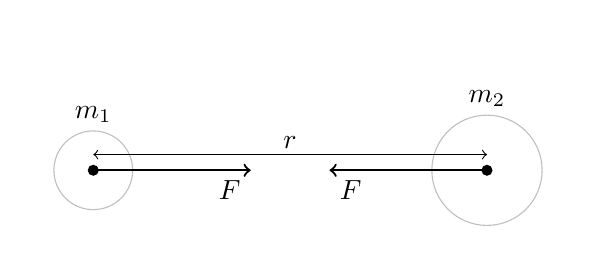
\begin{tikzpicture}
        \draw[lightgray] (0,0) circle (0.5cm) node[black,above,inner sep=0.6cm] {$m_1$};
        \draw[lightgray] (5,0) circle (0.7cm) node[black,above,inner sep=0.8cm] {$m_2$};
        \draw[->,thick] (0,0) -- (2,0) node[below left] {$F$};
        \draw[->,thick] (5,0) -- (3,0) node[below right] {$F$};
        \fill (0,0) circle[radius=2pt]; %node[below] {\tiny CM};
        \fill (5,0) circle[radius=2pt]; %node[below] {\tiny CM};
        \draw[<->] (0,0.2) -- (5,0.2);
        \node at (2.5,0.35) {$r$};
    \end{tikzpicture}
    %\caption{The model for Newton's law of universal gravitation.}
    \label{fig:Newton_Law_Universal_Gravitation}
    \end{center}

The equation for the law of gravitation is

\begin{equation} \label{eq:NLUG}
    F = \frac{G m_1 m_2}{r^2}
\end{equation}

\begin{center}
    \begin{tabular}{cl|cl}
    \hline
    \textbf{Symbol} & \textbf{Quantity} & \textbf{SI Base Unit} & \textbf{Unit Symbol}  \\
    \hline\hline
    \rule{0pt}{2.5ex}
        $F$ & gravitational force between two masses & Newton & N\\
        $G$ & gravitational constant & (\textit{see} $\rightarrow$) & \SI{}{N \cdot m^2/kg^2}\\
        $m_1$ & mass of object 1 & kilogram & kg\\
        $m_2$ & mass of object 2 & kilogram & kg\\
        $r$ & distance between centers of mass & meter & m\\
    \hline
    \end{tabular}
\end{center}

The \gls{GravConst} is always the same number (that's why it's a constant) and must be used any time the law of gravitation is applied. It's

\begin{equation*}
    G = \SI{6.67e-11}{\frac{N \cdot m^2}{kg^2}}
\end{equation*}
\end{mdframed}




\begin{example}
Consider two spheres of mass \SI{100.0}{kg} and \SI{400.0}{kg} whose centers are separated by \SI{4.00}{m}. What is the magnitude of the gravitational force between them?
\vspace{1ex}

\Solution We are given two masses and the distance between them: $m_1 = \SI{100.0}{kg}$, $m_2 = \SI{400}{kg}$, $r = \SI{4.00}{m}$. Also, remember that $G = \SI{6.67e-11}{N\,m^2/kg^2}$. By Newton's law of universal gravitation (Eq.~\ref{eq:NLUG}), the gravitational force is

\begin{equation*}
    F = \frac{G m_1 m_2}{r^2} = 
    \frac{\left(\SI{6.67e-11}{}\right) \left(100\right) \left(400\right)}{\left(4.00\right)^2} = 
    \SI{1.67e-7}{N}
\end{equation*}
\end{example}

\cyanhrule
\vspace{2ex}

Calculate the magnitude of the gravitational force between two objects.

\begin{exercise} \label{9DkhbB}
Two objects of mass \SI{707}{kg} and \SI{279}{kg} are separated by \SI{12}{m}. 
\end{exercise}



\begin{exercise} \label{MMnbpt}
What is the gravitational force between the objects below?
\vspace{-2em}

\begin{center}
    \centering
    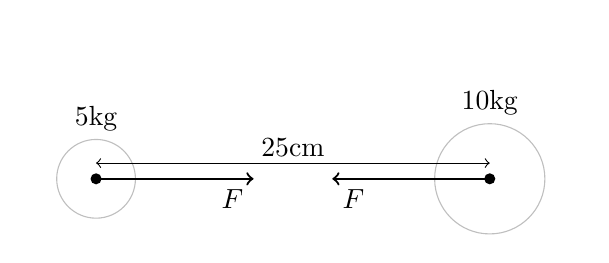
\begin{tikzpicture}
        \draw[lightgray] (0,0) circle (0.5cm) node[black,above,inner sep=0.6cm] {\SI{5}{kg}};
        \draw[lightgray] (5,0) circle (0.7cm) node[black,above,inner sep=0.8cm] {\SI{10}{kg}};
        \fill (0,0) circle (2pt); %node[below] {\tiny CM};
        \fill (5,0) circle (2pt); %node[below] {\tiny CM};
        \draw[<->] (0,0.2) -- (5,0.2);
        \node at (2.5,0.4) {\SI{25}{cm}};
        \draw[->,thick] (0,0) -- (2,0) node[below left] {$F$};
        \draw[->,thick] (5,0) -- (3,0) node[below right] {$F$};
    \end{tikzpicture}
\end{center}
\end{exercise}

\begin{example}
    The magnitude of the gravitational force that a 620-kg sphere and a 890-kg one exert on each other is \SI{7.52e-7}{N}. What is the distance between the spheres?
\end{example}

\Solution We are given two masses and the gravitational force: $m_1 = \SI{620}{kg}$, $m_2 = \SI{890}{kg}$, and $F = \SI{7.52e-7}{N}$. We are solving for distance: $r=$ ? These quantities are related by Newton's law of universal gravitation:

\begin{equation*}
    F = \frac{G m_1 m_2}{r^2}
\end{equation*}

To solve this equation for distance $r$, we take the following steps:

\begin{align*}
    \hspace{-3.5em} & \textbf{Substitute given values} & \hspace{-3em} &
    \SI{7.52e-7}{} = \frac{
        \left(\SI{6.67e-11}{}\right)
        \left(620\right)
        \left(890\right)
    }{r^2}
\end{align*}

\begin{align*}
    \hspace{-3.5em} & \textbf{Simplify} & \hspace{-3em} &
    \SI{7.52e-7}{} = \frac{\SI{3.68e-5}{}}{r^2}
\end{align*}

\begin{align*}
    \hspace{-3.5em} & \textbf{Re-write} & \hspace{-3em} &
    \frac{\SI{7.52e-7}{}}{1} = \frac{\SI{3.68e-5}{}}{r^2}
\end{align*}

\begin{align*}
    \hspace{-3.5em} & \textbf{Swap terms} & \hspace{-3em} &
    \frac{r^2}{1} = \frac{\SI{3.68e-5}{}}{\SI{7.52e-7}{}}
\end{align*}


\begin{align*}
    \hspace{-3.5em} & \textbf{Simplify} & \hspace{-3em} &
    r^2 = 48.9
\end{align*}

\begin{align*}
    \hspace{-3.5em} & \textbf{Take the square root} & \hspace{-3em} &
    \sqrt{r^2} = \sqrt{48.9}
\end{align*}

\begin{align*}
    \hspace{-3.5em} & \textbf{Therefore:} & \hspace{-3em} &
    r = \SI{7.00}{m}
\end{align*}


\begin{exercise} \label{dKPTLZ}
The gravitational force between two planetary bodies is \SI{2.52e20}{N}. The bodies' masses are \SI{3.9e23}{kg} and \SI{1.4e24}{kg}. What is the distance between the objects?
\end{exercise}


\hrule

\begin{exercise} \label{zw3NbF}
What is the distance between the objects below?

\begin{center}
    \centering
    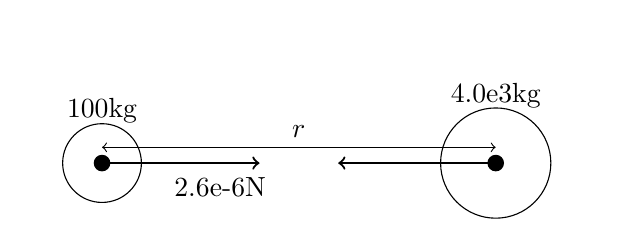
\begin{tikzpicture}
        \fill (0,0) circle[radius=3pt]; %node[below] {\tiny CM};
        \fill (5,0) circle[radius=3pt]; %node[below] {\tiny CM};
        \draw[<->] (0,0.2) -- (5,0.2);
        \node at (2.5,0.4) {$r$};
        \draw (0,0) circle (0.5cm) node[above,inner sep=0.5cm] {\SI{100}{kg}};
        \draw (5,0) circle (0.7cm) node[above,inner sep=0.7cm] {\SI{4.0e3}{kg}};
        \draw[->,thick] (0,0) -- (2,0);
        \draw[->,thick] (5,0) -- (3,0) ;
        \node at (1.5,-0.3) {\SI{2.6e-6}{N}};
        % \node at (3.8,-0.25) {$F$};
    \end{tikzpicture}
\end{center}
\end{exercise}

\cyanhrule

\subsection{Factor of Change Method}

The \textbf{factor of change method} allows you to calculate proportional changes in the gravitational force with proportional changes in distance and/or mass. Let Let $F$ be the original force and $F'$ be the changed force. The factors of change get plugged into the corresponding parentheses below:

\begin{equation*}
    \frac{F'}{F} \sim \frac{G m_1 m_2}{r^2} \sim \frac{(1)(\ )(\ )}{(\ )^2}
\end{equation*}

The two basic rules are summarized as follows:

\begin{enumerate}
\setlength\itemsep{0ex}
    \item If a quantity stays constant, plug in a 1 in the place where that quantity appears in the equation. Since $G$ is a constant, always plug in 1 for $G$.
    \item If a quantity changes by a factor other than 1, plug that factor in the equation. (For example, if distance doubles, plug in a 2 in the place of $r$.)
\end{enumerate}



\begin{example} \label{ex5bd1}
Two spheres are separated by 18 meters, and the gravitational force between them is \SI{3.0e-7}{N}. (a) If the distance between the objects is halved (changed to 9 meters), by what factor does the gravitational force change? (b) What is the new magnitude of the gravitational force?
\end{example}

\Solution Since the objects get closer, we expect the gravitational force to increase. Distance changes from \SI{18}{m} to \SI{9}{m}, implying that $r$ \textit{decreases} by a factor of 2. In other words, $r$ changes factor of $\frac{1}{2}$. All other factors stay constant. 

\begin{equation*}
    \frac{F^{\prime}}{F} \sim \frac{G m_1 m_2}{r^2} \sim \frac{(1)(1)(1)}{\left(\frac{1}{2}\right)^2} = \frac{1}{\left(\frac{1}{4}\right)} = 4
\end{equation*}

This means $F'$ is 4 times greater than the original force $F$, as we expected:

\begin{equation*}
    F' = 4 F = 4 \times  \left(\SI{3.0e-7}{N}\right) = \SI{1.2e-6}{N}
\end{equation*}


\vspace{1em}
\hrule

\begin{example}
If the distance in Example~\ref{ex5bd1} \textit{increases} by 2 rather than decreases, what is the proportional change in the gravitational force?
\end{example} 

\Solution Now $r$ changes by a factor of 2, and $m_1$ and $m_2$ continue staying the same:

\begin{equation*}
    \frac{F^{\prime}}{F} \sim \frac{G m_1 m_2}{r^2} \sim \frac{(1)(1)(1)}{(2)^2} = \frac{1}{2^2} =\frac{1}{4}
\end{equation*}

$F'$ will decrease to $\frac{1}{4}$ the magnitude of $F$.

\vspace{1ex}
\cyanhrule
\vspace{1ex}

The gravitational force, as shown in the previous examples, is known as an ``inverse-square law,'' since force scales as 1 over the distance squared:

\begin{equation*} \tag{inverse-square law}
    F \sim \frac{1}{r^2} \hspace{3em}
\end{equation*}

\begin{exercise} \label{WhkfQ4}
By what factor does the gravitational force $F$ change if the distance $r$ is increases to $3r$? (See Figure~\ref{fig:Newton_Law_Universal_Gravitation}.) 
\end{exercise}

\begin{exercise} \label{CqOs7y}
By what factor does the gravitational force $F$ change if the distance $r$ is changes to 10\% of $r$? 
\end{exercise}

\begin{exercise} \label{PwaIbN}
By what factor does the gravitational force between two objects change when the distance between them \textit{increases} by a factor of 4?
\end{exercise}

\begin{exercise} \label{akw9Hx}
By what factor does the gravitational force between two objects change when the distance between them \textit{decreases} by a factor of 4?
\end{exercise}

\begin{exercise} \label{Dhfy9M}
By what factor does the gravitational force between two objects change when the distance between them \textit{increases} by a factor of 5?
\end{exercise}

\begin{exercise} \label{gjeHTU}
By what factor does the gravitational force between two objects change when the distance between them \textit{decreases} by a factor of 5?
\end{exercise}

\begin{exercise} \label{yXaSNL}
Calculate Earth's tangential speed in its orbit around the Sun. Assume that the centripetal force on Earth is the gravitational force exerted on Earth by the Sun. The mass of the Sun is \SI{1.99e30}{kg}, and the average distance between Earth and the Sun is \SI{1.5e11}{m}.
\end{exercise}

\cyanhrule
\clearpage
\subsection{Acceleration due to gravity}

\begin{example}
Show that an object of any mass $m$ that is in free-fall near the surface of Earth will accelerate downwards due to gravity at a rate of $g = \SI{9.8}{m/s^2}$. You'll need the planetary data summarized below:

\begin{center}
    \centering
    \begin{tabular}{c|c}
        \textbf{Earth's mass} & \textbf{Earth's radius} \\
        \hline
        \SI{5.9736e24}{kg} & \SI{6.376e6}{m}\\
    \end{tabular}
\end{center}
\end{example}

\Solution Let's re-write Newton's Law of Universal Gravitation (Eq.~\ref{eq:NLUG}) as

\begin{equation*}
    F = \frac{G m M}{R^2}\ ,
\end{equation*}

where $M = \SI{5.97e24}{kg}$ is Earth's mass, and $R = \SI{6.38e6}{m}$ is Earth's radius. The distance between the centers of mass of Earth and object $m$ is Earth's radius, as the picture below depicts:

% \begin{equation*}
%     r = R_{\mathrm{\Earth}} = \SI{6.376e6}{m}.
% \end{equation*}

\begin{center}
    \centering
    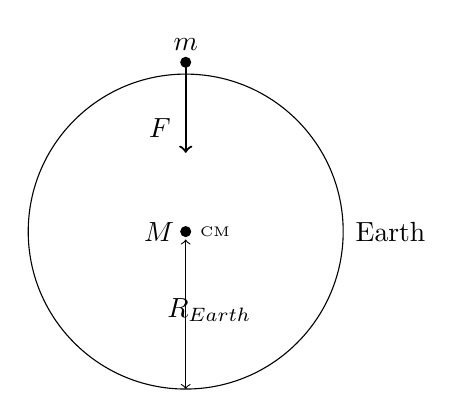
\begin{tikzpicture}
        \fill (0,0) circle (2pt) node[right,inner sep=5pt] {\tiny CM};
        \draw[<->] (0,-0.1) -- (0,-2);
        \draw[->,thick] (0,2.1) -- (0,1) node[anchor=south east,inner sep = 5pt] {$F$};
        \node at (0.3,-1) {$R_{\text{Earth}}$};
        \draw (0,0) circle (2cm) node[left,inner sep=4pt] {$M$};
        \fill (0,2.15) circle (2pt) node[above,inner sep = 4pt] {$m$};
        \node at (2.6,0) {Earth};
    \end{tikzpicture}
\end{center}

Recall that Newton's Second Law of Motion (from Unit 4) states

\begin{equation*}
    F_{\text{net}} = m a
\end{equation*}

The only force on $m$ is the gravitational force from Earth. Combining Newton's 2nd Law with Newton's Law of Universal Gravitation leads to

\begin{equation*}
    F = ma = \frac{G m M}{R^2}
\end{equation*}

Since mass $m$ appears on both sides of the equation, it cancels:

\begin{equation*}
    \textcolor{red}{\cancel{m}}a = \frac{G \textcolor{red}{\cancel{m}} M}{R^2}
\end{equation*}

leaving only

\begin{equation*}
    a = \frac{G M}{R^2}
\end{equation*}

When planetary mass and radius are plugged in, this acceleration is defined as \textit{acceleration due to gravity}, $g$, near the planet's surface:

\begin{equation}
    g = \frac{GM}{R^2}
\end{equation}


Plugging in Earth's mass and radius leads to 

\begin{equation*} 
    g = \frac{GM}{R^2} = \frac{\left(\SI{6.674e-11}{}\right)\left(\SI{5.97e24}{}\right)}{\left(\SI{6.38e6}{m}\right)^2} = \SI{9.81}{m/s^2}
\end{equation*}


\begin{exercise} \label{knMwSV}
The Moon is about 384,000 kilometers away. What is the acceleration due to gravity from Earth at the halfway point to the Moon? 
\end{exercise}

\hrule

\ref{B208cB}--\ref{416pje} Calculate (a) centripetal acceleration and (b) centripetal force for an object in uniform circular motion for the given quantities.

\begin{exercise} \label{B208cB}
mass is \SI{45}{kg}, tangential speed is \SI{7}{m/s}, radius of curvature is \SI{10}{m}
\end{exercise}

\begin{exercise}
tangential speed is \SI{18}{m/s}, mass is \SI{2000}{kg}, radius of curvature is \SI{24}{m}
\end{exercise}

\begin{exercise}
radius of curvature is \SI{3}{m}, mass is \SI{842}{kg}, tangential speed is \SI{92}{m/s}
\end{exercise}

\begin{exercise}
radius of curvature is \SI{45}{m}, tangential speed is \SI{15}{m/s}, mass is \SI{1961}{kg}
\end{exercise}

\begin{exercise}\label{416pje}
tangential speed is \SI{6}{m/s}, radius of curvature is \SI{20}{m}, mass is \SI{1540}{kg}
\end{exercise}

% \textit{Solution}

% \textbf{Known}: $h = \SI{384000}{km} = \SI{3.84e8}{m}$, $M = \SI{5.9736e24}{kg}$, $R_{\mathrm{\Earth}} = \SI{6.376e6}{m}$

% Then

% \begin{equation*}
%     g = \frac{GM}{r^2} = \frac{G M}{\left(R_{\Earth} + h\right)^2} = \SI{0.010}{m/s^2}
% \end{equation*}

\subsection{Answers}
\ref{9DkhbB}. \SI{9.14e-8}{N}\\
\ref{MMnbpt}. \SI{5.3e-8}{N}\\
\ref{zw3NbF}. \SI{3.2}{m}\\
\ref{knMwSV}. \SI{0.010}{m/s^2}\\
\ref{WhkfQ4}. $\frac{1}{9}$\\
\ref{CqOs7y}. 100\\
\ref{PwaIbN}. $\frac{1}{16}$\\
\ref{akw9Hx}. 16\\
\ref{Dhfy9M}. $\frac{1}{25}$\\
\ref{gjeHTU}. 25\\
\ref{yXaSNL}. \SI{2.98e4}{m/s} ($\approx \SI{30}{km/s}$)\\
\ref{dKPTLZ}. \SI{3.8e8}{m}\\



\clearpage
\printnoidxglossaries


\clearpage

\section{Projectile Motion}




\begin{example} \label{4Dn9PW}
    During a fireworks display like the one illustrated in Figure \ref{ZxjpEr}, a shell is shot into the air with an initial speed of \SI{70.0}{m/s} at an angle of \ang{75} above the horizontal. The fuse is timed to ignite the shell just as it reaches its highest point above the ground. Calculate the height at which the shell explodes. (This peak vertical position is defined as \gls{maximum height}.)
\end{example}

\begin{center}
    \begin{tikzpicture}[
        declare function={f(\x)=\yi + tan(\thetai)*\x - \grav*\x^2/(2*(\vi*cos(\thetai))^2);},
        declare function={t(\x)=\x/(\vi*cos(\thetai));}
    ]
    \tikzmath{
        \grav = 9.8;
        \vi = 70;
        \yi = 0.0;
        \thetai = 75.0;
        \viy = \vi*sin(\thetai);
        \ymax = (\viy^2)/(2*\grav);
        \tmax = 2*\ymax/\viy;
        \vix = \vi*cos(\thetai);
        \xmax = \vix*\tmax;
        \sf = 0.25; %scale factor for vector components
    }
    \pgfplotsset{compat=1.11}
        \begin{axis}[width=8cm,height=8cm,ticks=none,
        axis lines = center,
        clip=false,
        ylabel = $y$,
        xlabel = $x$,
        xmin=0, xmax=175,
        ymin=0, ymax=275,
        ]
        \draw[domain=0:\xmax,variable=\x,samples=250] plot ({\x},{f(\x)});
        \draw (10,0) arc (0:35:30) node[pos=0.8,right=2pt] {$\theta = \ang{75}$};
        \draw[dashed] (0,\ymax) node[left] {$h$} -- ++(\xmax,0);
        \draw[dashed] (\xmax,0) -- ++(0,\ymax);
        \draw[ultra thick,violet,->] (0,0) -- ++({\vi*cos(\thetai)},{\vi*sin(\thetai)}) node[left] {$v$};
        \end{axis}
    \end{tikzpicture}
    \captionsetup{type=figure,margin=1in,font=scriptsize}
    \captionof{figure}{The diagram shows the trajectory of a fireworks shell.}
    \label{ZxjpEr}
\end{center}

\Solution We are given the initial speed and launch angle: $v_0 = \SI{70}{m/s}$ and $\theta_0 = \ang{75}$. We know the magnitude of the acceleration due to gravity is $g = \SI{9.8}{m/s^2}$. Since horizontal and vertical motions are independent, we start by analyzing only the vertical motion. The $y$-component of the initial velocity is given by

\begin{equation*}
    v_{0y} = v_0 \sin{\theta_0} = 70 \sin{(\ang{75})} = 67.61
\end{equation*}

If we assume the firework starts at the origin, its initial vertical position is zero: $y_0 = 0$.

\vspace{1em}

The unknown we are looking for is final vertical position (or height above $y_0$): $y =\ ?$ 

\vspace{1em}

The key to solving this problem is the following fact: From Figure ?.?? we see that at the highest point in the trajectory, the $y$-component of velocity is zero: $v_y = 0$. Therefore, at the highest point, the given and unknown quantities are related by Equation \eqref{wROSXN}:

\begin{equation*}
    v_y^2 = v_{0y}^2 - 2 g \left(y-y_0\right)
\end{equation*}

Substituting known values leads to

\begin{equation*}
    0^2 = \left(67.6\right)^2 - 2 (9.8) \left(y - 0\right)
\end{equation*}

or, more simply, to

\begin{equation*}
    0 = 67.6^2 - 19.6 y
\end{equation*}

We can solve this equation for height $y$ as follows:

\begin{align*}
    \textbf{Add $19.6 y$} \qquad & 0 \redplus \textcolor{red}{19.6 y} = 67.6^2 - \cancel{19.6 y} \redplus \textcolor{red}{\cancel{19.6 y}}\\[1ex]
    \textbf{Simplify} \qquad & 19.6 y = 67.6^2\\[1ex]
    \textbf{Divide by 19.6} \qquad & \frac{\cancel{19.6} y}{\textcolor{red}{\cancel{19.6}}} = \frac{67.6^2}{\textcolor{red}{19.6}}\\[1ex]
    \textbf{Simplify} \qquad & y = 233
\end{align*}

Therefore, the maximum height of the firework is 233 meters.

\endsolution

\begin{example} \label{t57osh}
    How much time passed between the launch of the shell in Example \ref{4Dn9PW} and the explosion?
\end{example}

\Solution
Upon solving Example \ref{4Dn9PW}, we learned that initial and final vertical velocities associated with a launch to maximum height are

\begin{equation*}
    v_{0y} = \SI{67.6}{m/s} \quad \text{and} \quad v_y = \SI{0}{m/s}
\end{equation*}

Furthermore, gravitational acceleration is always $g = \SI{9.8}{m/s^2}$. Since we are now looking for how long it took the firework to reach maximum height, the unknown is time: $t =\ ?$

\vspace{1em}

The given and unknown quantities are now related by Equation \eqref{SjYaoE} as 

\begin{equation*}
    v_y = v_{0y} - gt
\end{equation*}

Substituting known values leads to

\begin{equation*}
    0 = 67.6 - 9.8 t
\end{equation*}

Let's solve this equation as follows:

\begin{align*}
    \textbf{Add $9.8 t$} \qquad & 0 \redplus \textcolor{red}{9.8 t} = 67.6 - \cancel{9.8 t} \redplus \cancel{\textcolor{red}{9.8 t}}\\[1ex]
    \textbf{Simplify} \qquad & 9.8 t = 67.6\\[1ex]
    \textbf{Divide by 9.8} \qquad & \frac{\cancel{9.8} t}{\cancel{\textcolor{red}{9.8}}} = \frac{67.6}{\textcolor{red}{9.8}}\\[1ex]
    \textbf{Simplify} \qquad & t = 6.90
\end{align*}

Therefore, from the launch of the firework to its explosion at maximum height, a total of 6.90 seconds elapsed.

\endsolution

\begin{example} 
    What is the horizontal displacement of the shell in Example \ref{4Dn9PW} when it explodes?
\end{example}

\Solution In this example, since we are asked to find horizontal displacement, we analyze only the horizontal motion. Assuming the firework is launched from the origin, its initial position is $x_0 = 0$. Since the initial speed and launch angle are $v_0 = \SI{70}{m/s}$ and $\theta_0 = \ang{75}$,  the horizontal component of initial velocity is

\begin{equation*}
    v_{0x} = v_0 \cos{\theta_0} = 70 \cos{(\ang{75})} = \SI{18.1}{m/s}
\end{equation*}

In horizontal motion, by Equation \eqref{dCvDf4}, velocity is a constant, meaning that the projectile, throughout its trajectory, will maintain a constant horizontal speed of 

\begin{equation*}
    v_x = v_{0x} = \SI{18.1}{m/s}
\end{equation*}


Furthermore, in Example \ref{t57osh}, we concluded that the time from launch to maximum height is $t = \SI{6.90}{s}$. Finally, the unknown we are looking for is displacement from the origin: $x =\ ?$.

\vspace{1em}

The known and unknown quantities are related by Equation \eqref{7fMAPG} as

\begin{equation*}
    x = x_0 + v_x t
\end{equation*}

Substituting known values leads to 

\begin{equation*}
    x = 0 + (18.1)(6.90) = 125 
\end{equation*}

Therefore, the firework was horizontally displaced by 125 meters.

\endsolution

\begin{example}
    \href{https://youtu.be/9Ijev8RHF04}{Brynden the Blackfish} uses a bow to launch an arrow at a speed of \SI{39}{m/s}. The arrow's trajectory looks like those shown in Figure \ref{6hKQ2Y}. If the launch angle is \ang{56}, what is the arrow's range? Ignore air resistance (which, actually, \textit{could} affect the motion of the arrow.) 
\end{example}

\Solution We are given the initial speed and launch anlge: $v_0 = \SI{39}{m/s}$ and $\theta_0 = \ang{56}$. Acceleration due to gravity always has a magnitude of $g = \SI{9.8}{m/s^2}$. 

\vspace{1em}

The unknown we are looking for is range, which is given by Equation \eqref{GqvaN1} as

\begin{equation*}
    R = \frac{v_0^2 \sin{2\theta_0}}{g}
\end{equation*}

Substituting known values leads to

\begin{equation*}
    R = \frac{39^2 \sin{(2 \cdot \ang{56})}}{9.8} = 144
\end{equation*}

Therefore, the range of the arrow is 144 meters. That's how far it can travel horizontally.

\endsolution

\begin{example} \label{9XXF9X}
    George drops a rock from rest from the top of an \SI{82}{m} tall cliff. Calculate how long it will take the rock to impact the ground. 
\end{example}

\Solution We are given the rock's initial velocity (``from rest''): $v_{0y} = 0$. Taking the rock's initial vertical position to be the origin, then we are also given its initial and final positions: $y_0 = 0$ and $y = \SI{-82}{m}$. Furthermore, we know the magnitude of gravitational acceleration is $g = \SI{9.8}{m/s^2}$. 

\vspace{1em}

The unknown we are looking for is time: $t =\ ?$

\vspace{1em}

The given and unknown quantities are related by Equation \eqref{36YuvF}:

\begin{equation*}
    y = y_0 + v_{0y}t - \frac{1}{2}  g t^2
\end{equation*}

Substituting given values leads to 

\begin{equation*}
    -82 = 0 + (0) t - \frac{1}{2} g t^2
\end{equation*}

or, more simply, to

\begin{equation*}
    -82 = - 4.9 t^2
\end{equation*}

Since we are solving this equation for time, $t$, we should write the unknown variable on the left:

\begin{equation*}
    -4.9 t^2 = -82
\end{equation*}

This equation is solved as follows:

\begin{align*}
    \textbf{Divide by $-4.9$} \qquad & \frac{\cancel{-4.9} t^2}{\cancel{\redminus \textcolor{red}{4.9}}} = \frac{-82}{\redminus \textcolor{red}{4.9}}\\[1ex]
    \textbf{Simplify} \qquad & t^2 = \frac{82}{4.9}\\[1ex]
    \textbf{Take square root} \qquad & \sqrt{t^2} = \sqrt{\frac{82}{4.9}}\\[1ex]
    \textbf{Simplify} \qquad & t = 4.09
\end{align*}

Therefore, dropping from rest, it takes this rock 4.09 seconds to strike the ground.

\endsolution


\begin{example} \label{lB7EDG}
    A cannon is aimed at a right angle to the horizontal, perfectly upwards, next to a 76-meter-tall redwood tree. The cannon fires a cannonball at a speed of \SI{42}{m/s}. How much time after launch does it take the cannonball to reach the top of the tree, if the projectile has passed maximum height and is on its way down?
\end{example}

\Solution Since the cannonball's motion is strictly vertical, we will work with equations governing vertical motion only. We are given the cannonball's initial speed: $v_{0y} = \SI{42.0}{m/s}$. Gravitational acceleration always has a magnitude of $g = \SI{9.80}{m/s^2}$. If we assume the cannonball starts at the origin, then we know its initial and final positions: $y_0 = 0$ and $y = \SI{76.0}{m}$. The unknown we are looking for is the time: $t =\ ?$.

\vspace{1em}

The given and unknown quantities are related by Equation \eqref{36YuvF}:

\begin{equation*}
    y = y_0 + v_{0y}t - \frac{1}{2}  g t^2
\end{equation*}

Substituting given values leads to 

\begin{equation*}
    76 =  0 + 42 t -\frac{1}{2}(9.8) t^2\ ,
\end{equation*}

or, more simply, to

\begin{equation*}
    76 = 42 t - 4.9 t^2
\end{equation*}

We may solve for time, $t$, as follows:

\begin{align*}
    \textbf{Add $4.9 t^2$} \qquad & 76 \redplus \textcolor{red}{4.9 t^2} = 42 t - 4.9 t^2 \redplus \textcolor{red}{4.9 t^2}\\[1ex]
    \textbf{Simplify} \qquad & 76 + 4.9 t^2 = 42 t\\[1ex]
    \textbf{Subtract $42 t$} \qquad & 76 + 4.9 t^2 \redminus \textcolor{red}{42 t} = 42 t \redminus \textcolor{red}{42 t}\\[1ex]
    \textbf{Simplify} \qquad & 76 + 4.9 t^2 - 42 t = 0
\end{align*}

The last equation may be rearranged as 

\begin{equation} \label{LScbXD}
    4.9 t^2 - 42 t + 76 = 0
\end{equation}

so that it resembles the quadratic form

\begin{equation} \label{WsGUny}
    ax^2 + bx + c = 0
\end{equation}

whose two solutions are given by the quadratic equation

\begin{equation} \label{BMWMHy}
    x = \frac{-b \pm \sqrt{b^2 - 4ac}}{2a}
\end{equation}

Setting the coefficients in Equation \eqref{LScbXD} to match the symbols in Equation \eqref{WsGUny} leads to 

\begin{equation*}
    a = 4.9\ , \quad b = -42\ ,\quad c = 76
\end{equation*}

Substituting these coefficients into Equation \eqref{BMWMHy} leads to the first solution of time:

\begin{equation*}
    t_1 = \frac{-b + \sqrt{b^2 - 4ac}}{2a} = \frac{-(-42) + \sqrt{(-42)^2 - 4 (4.9)(76)}}{2(4.9)} = \SI{5.98}{s}
\end{equation*}

Likewise, the second solution of time is given by

\begin{equation*}
    t_2 = \frac{-b - \sqrt{b^2 - 4ac}}{2a} = \SI{2.60}{s}
\end{equation*}

Since the second solution, $t_2 = \SI{2.60}{s}$, is less than the first, it must correspond to the cannonball reaching the top of the tree ($y=\SI{76}{m}$) on the way \textit{up}. The first solution ($t_1 = \SI{5.98}{s}$) corresponds to the projectile reaching the same point on its way back down. Therefore, the cannonball will reach the top of the tree, on its way back down, 5.98 seconds after the initial launch.

\endsolution


\begin{example} \label{pyn6Go}
    George, from Example \ref{9XXF9X}, this time throws a rock downwards at a speed of \SI{17.00}{m/s} from the top of the same \SI{82}{m} tall cliff. Calculate how long it will take the rock to impact the ground now.
\end{example}

\Solution We are given initial velocity: $v_{0y} = \SI{-17.00}{m/s}$. Assuming that the rock's initial vertical position is zero, then we are given the following initial and final positions: $y_0 = 0$ and $y = \SI{-82}{m}$. Also, we know the magnitude of gravitational acceleration is always $g = \SI{9.8}{m/s^2}$. 

\vspace{1em}

The unknown we are looking for is time: $t =\ ?$

\vspace{1em}

The given and unknown quantities are related by Equation \eqref{36YuvF}:

\begin{equation*}
    y = y_0 + v_{0y}t - \frac{1}{2}  g t^2
\end{equation*}

This is the same equation and unknown that was referred to in Example \ref{lB7EDG}, so the current solution will develop almost exactly like the one from Example \ref{lB7EDG}, even though the two examples involve different trajectories.


\vspace{1em}

Substituting given values leads to 

\begin{equation*}
    -82 =  0 - 17 t -\frac{1}{2}(9.8) t^2\ ,
\end{equation*}

or, more simply, to

\begin{equation*}
     -82 = - 17 t -4.9 t^2
\end{equation*}

Let's rearrange this equation as follows:

\begin{align*}
    \textbf{Add $17t$} \qquad & - 82 \redplus \textcolor{red}{17t} = -17t \redplus \textcolor{red}{17t} - 4.9 t^2 \\[1ex]
    \textbf{Simplify} \qquad & -82 + 17t = -4.9t^2\\[1ex]
    \textbf{Add $4.9 t^2$} \qquad & -82 + 17t \redplus \textcolor{red}{4.9 t^2} = -4.9t^2 \redplus \textcolor{red}{4.9 t^2}\\[1ex]
    \textbf{Simplify} \qquad & -82 + 17t + 4.9t^2 = 0
\end{align*}

The last equation is rearranged as 

\begin{equation} \label{dw27jh}
    4.9 t^2 + 17t - 82 = 0
\end{equation}

so that it fits the quadratic form $ax^2 + bx + c = 0$, which has two solutions given by the quadratic equation \eqref{BMWMHy}. Let the coefficients in Equation \eqref{dw27jh} be

\begin{equation*}
    a = 4.9\ , \quad b = 17\ ,\quad c = -82
\end{equation*}

so that the first root of time is

\begin{equation*}
    t_1 = \frac{-b + \sqrt{b^2 - 4ac}}{2a} = \frac{-17 + \sqrt{17^2 - 4(4.9)(-82)}}{2(4.9)} = \SI{2.71}{s}
\end{equation*}

The second solution is found similarly as

\begin{equation*}
    t_2 = \frac{-b - \sqrt{b^2 - 4ac}}{2a} = \SI{-6.18}{s}
\end{equation*}

Since the rock must strike the ground \textit{after} it is thrown, we take the first solution of time as the answer to this exercise: the rock strikes the ground 2.71 seconds after it is launched. 

\endsolution

\begin{example}
    Suppose a large rock is ejected from a volcano, as illustrated in Figure ?.??, with a speed of  \SI{25.0}{m/s} and at an angle \ang{35} above the horizontal. The rock strikes the side of the volcano at an altitude 20.0 m lower than its starting point. Calculate the time it takes the rock to follow this path.
\end{example}

\begin{center}
    \begin{tikzpicture}[
        declare function={f(\x)=\yi + tan(\thetai)*\x - \grav*\x^2/(2*(\vi*cos(\thetai))^2);},
        declare function={t(\x)=\x/(\vi*cos(\thetai));}
    ]
    \tikzmath{
        \grav = 9.8;
        \vi = 25;
        \yi = 0.0;
        \thetai = 35.0;
        \viy = \vi*sin(\thetai);
        \ymax = (\viy^2)/(2*\grav);
        \tmax = 2*\ymax/\viy;
        \vix = \vi*cos(\thetai);
        \xmax = \vix*3.96; %t = 3.96 s
        \sf = 0.5; %scale factor for vector components
    }
    \pgfplotsset{compat=1.11}
        \begin{axis}[width=12cm,height=7cm,ticks=none,
        axis lines = center,
        clip=false,
        ylabel = $y$,
        xlabel = $x$,
        xmin=0, xmax=100,
        ymin=-30, ymax=10,
        ]
        \draw[domain=0:\xmax,variable=\x,samples=250] plot ({\x},{f(\x)});
        \draw[ultra thick,violet,->] (0,0) -- ++(axis direction cs: {\sf*\vix},{\sf*\viy}) node[above=-1pt] {$\SI{25}{m/s}$};
        \draw (5,0) arc (0:35:5) node[pos=0.1,right=-1pt] {\ang{35}};
        \draw[dashed] (\xmax,-20) -- ++(axis direction cs: 0,20) node[pos=0.5,right] {-\SI{20}{m}};
        \draw[fill=black] (\xmax,-20) circle (2pt);
        \draw (\xmax,-20) -- ++(axis direction cs: 12,0);
        \draw[,ultra thick,->,violet] (\xmax,-20) -- ++(axis direction cs: {\sf*\vix},{\sf*(\viy -\grav*3.96)}) node[below=-2pt] {$v$};
        \draw (\xmax+5,-20) arc (0:-48:5) node[pos=0.1,right=-1pt] {$\theta$};
        \end{axis}
    \end{tikzpicture}
    \captionsetup{type=figure,margin=1in,font=scriptsize}
    \captionof{figure}{The diagram represents the projectile motion of a large rock from a volcano.}
\end{center}

\Solution Recall the most important concept in projectile motion: horizontal and vertical motions are independent. Since they don't influence one another, we can analyze them separately. For this problem, we can ignore calculations related to the horizontal motion and focus only on the vertical motion. As such, the solution to this example will develop like Examples \ref{lB7EDG} and \ref{pyn6Go}. 

\vspace{1em}

We are given the initial speed and launch angle: $v_0 = \SI{25.0}{m/s}$ and $\theta_0 = \ang{35}$. If we set the origin to be the rock's initial position, then the initial and final vertical positions are $y_0 = 0$ and $y = \SI{-20.0}{m}$. The magnitude of gravitational acceleration is $g = \SI{-9.8}{m/s^2}$.

\vspace{1em}

Since we are analyzing vertical motion only, we get the $y$-component of initial velocity by

\begin{equation*}
    v_{0y} = v_0 \sin{\theta_0} = 25 \sin{(\ang{35})} = 14.34
\end{equation*}

 The unknown quantity we are looking for is time: $t =\ ?$ These given and unknown quantities are related by Equation \eqref{36YuvF}

\begin{equation*}
    y = y_0 + v_{0y}t - \frac{1}{2} g t^2
\end{equation*}

At this point, this example is solved like the solutions to Examples \ref{lB7EDG} and \ref{pyn6Go}. As shown previously, we can define the coefficients $a$, $b$, and $c$ to fit the given quantities from this example. Then, applying the quadratic formula \eqref{BMWMHy} with those coefficients leads to the two solutions (roots) of time:

\begin{equation*}
    t_1 = \SI{3.96}{s} \quad \text{and} \quad t_2 = \SI{-1.03}{s}
\end{equation*}

Choosing the positive solution, we conclude that the rock will strike the ground 3.96 seconds after launch.

\subsubsection*{Range (K-level only)}

The fact that vertical and horizontal motions are independent of each other lets us predict the range of a projectile. The \gls{range} is the horizontal distance $R$ traveled by a projectile on level ground, as illustrated in Figure \ref{6hKQ2Y}. Throughout history, people have been interested in finding the range of projectiles for practical purposes, such as aiming cannons.

\begin{center}
    \begin{tikzpicture}[
        declare function ={R(\vi,\thetai)= \vi^2*sin(2*\thetai)/\grav;}, %range
        declare function={h(\vi,\thetai)=(\vi*sin(\thetai))^2/(2*\grav);}, %maximum height
    ]
    \tikzmath{
        \grav = 9.8;
        \sf = 0.5; %scale factor for vector components
    }
    \pgfplotsset{compat=1.11}
        \begin{axis}[width=12cm,height=5cm,ticks=none,
        axis lines = center,
        clip=false,
        ylabel = $y$,
        xlabel = $x$,
        xmin=0, xmax={R(50,45)*1.1},
        ymin=0, ymax={h(50,45)*1.1},
        ]
        \draw[Green,thick,->] (0,0) -- ++({50*cos(45)},{50*sin(45)}) node[above left=-5pt] {\SI{50}{m/s}};;
        \draw[Green,thick,domain=0:{R(50,45)},variable=\x,samples=250] plot ({\x},{patheq(\x,0,50,45)}) node[black,below] {$R = \SI{225}{m}$};
        \draw[violet,thick,->] (0,0) -- ++({40*cos(45)},{40*sin(45)}) node[pos=0.93,right=2.7mm] {\SI{40}{m/s}};;
        \draw[violet,thick,domain=0:{R(40,45)},variable=\x,samples=250] plot ({\x},{patheq(\x,0,40,45)}) node[black,below] {$R = \SI{163}{m}$};
        \draw[red,thick,->] (0,0) -- ++({30*cos(45)},{30*sin(45)}) node[pos=0.4,right=3pt] {\SI{30}{m/s}, \ang{45}};
        \draw[red,thick,domain=0:{R(30,45)},variable=\x,samples=250] plot ({\x},{patheq(\x,0,30,45)})
    node[black,below] {$R = \SI{91.8}{m}$};;
        \end{axis}
    \end{tikzpicture}

    \vspace{1em}

    \begin{tikzpicture}[
        declare function ={R(\vi,\thetai)= \vi^2*sin(2*\thetai)/\grav;}, %range
        declare function={h(\vi,\thetai)=(\vi*sin(\thetai))^2/(2*\grav);}, %maximum height
    ]
    \tikzmath{
        \grav = 9.8;
        \sf = 0.5; %scale factor for vector components
    }
    \pgfplotsset{compat=1.11}
        \begin{axis}[width=12cm,height=5cm,ticks=none,
        axis lines = center,
        clip=false,
        ylabel = $y$,
        xlabel = $x$,
        xmin=0, xmax={R(50,45)*1.1},
        ymin=0, ymax={h(50,75)*1.1},
        ]
        \draw[Green,thick,->] (0,0) -- ++({50*cos(75)},{50*sin(75)}) node[pos=1.7,rotate=58] {\SI{50}{m/s}, \ang{75}};;
        \draw[Green,thick,domain=0:{R(50,75)},variable=\x,samples=250] plot ({\x},{patheq(\x,0,50,75)}) node[black,below] {$R = \SI{128}{m}$};
        \draw[violet,thick,->] (0,0) -- ++({50*cos(45)},{50*sin(45)}) node[pos=1.6,rotate=20,below=-6pt] {\SI{50}{m/s}, \ang{45}};;
        \draw[violet,thick,domain=0:{R(50,45)},variable=\x,samples=250] plot ({\x},{patheq(\x,0,50,45)}) node[black,below] {$R = \SI{225}{m}$};
        \draw[red,thick,->] (0,0) -- ++({50*cos(15)},{50*sin(15)}) node[pos=1.5] {\SI{50}{m/s}, \ang{15}};;
        \draw[red,thick,domain=0:{R(50,15)},variable=\x,samples=250] plot ({\x},{patheq(\x,0,50,15)});
        \end{axis}
    \end{tikzpicture}
    \captionsetup{type=figure,margin=1in,font=scriptsize}
    \captionof{figure}{Trajectories of projectiles on level ground. \textit{Top plot}: The greater the initial speed,$v_0$, the greater the range for a given initial angle. \textit{Bottom plot}: The effect of initial angle, $\theta_0$, on the range of a projectile with a given initial speed. Note that any combination of trajectories that add to 90 degrees will have the same range in the absence of air resistance, although the maximum heights of those paths are different.}
    \label{6hKQ2Y}
\end{center}

How does the initial velocity of a projectile affect its range? Obviously, the greater the initial speed $v_0$, the greater the range, as shown in the figure above. The initial angle $\theta_0$ also has a dramatic effect on the range. When air resistance is negligible, the range $R$ of a projectile on level ground is

\begin{equation} \label{GqvaN1}
    R = \frac{v_0^2 \sin{(2\theta_0)}}{g}
\end{equation}

where $v_0$ is the initial speed and $\theta_0$ is the initial angle relative to the horizontal. It is important to note that the range doesn't apply to problems where the initial and final $y$ position are different, or to cases where the object is launched perfectly horizontally.

\end{document}